\documentclass[10pt]{article}
\usepackage[utf8]{inputenc}
\usepackage[ngerman]{babel}
\usepackage{graphicx}
\usepackage{float}
%\usepackage{a4}
\usepackage[a4paper, left=2.5cm, right=2.5cm, top=2.5cm, bottom=2cm]{geometry}
% die Schrift ist bei Times New Roman kleiner, sieht aber auch nicht so gut aus
%\usepackage{mathptmx}

\usepackage[
 colorlinks=true,
urlcolor=blue,
linkcolor=black,
citecolor=blue
]{hyperref}

\usepackage[all]{hypcap}
\usepackage[table]{xcolor}

\usepackage[backend=biber, style=numeric, maxcitenames=5, maxbibnames=20, sorting=none, dateabbrev=false]{biblatex}% backend=biber, 
\addbibresource{Quellen.bib}
% oder
% \begin{filecontents*}{Literatur.bib}  
%  @TECHREPORT{001,    %KEY
%    author = {Hans Mustermann},  
%    title = {Einfach nur ein Titel},  
%    number = {ABCD-E/2008/de/1234},  
%    institution = {Firma AG},  
%    year = {2008}  
%  }   
%  \end{filecontents*} 

%\DeclareFieldFormat{urltime}{#1}
% \DeclareFieldFormat{date}{#1}    % Not sure with this one
% \DeclareFieldFormat{title}{#1\addcomma}
% \DeclareFieldFormat{url}{\newline\bibstring{URL}\addcolon\addspace\url{#1}}
% \DeclareFieldFormat{urltime}{#1}
% \DeclareFieldFormat{urldate}{\addcomma\space#1\addcomma\addspace\printfield{urltime}}

% kein Tab nach einem Bild
\setlength\parindent{0pt}


\usepackage{tocloft}
\usepackage{csquotes}


%Header
% \usepackage{fancyhdr}
% \pagestyle{fancy}
% \renewcommand{\sectionmark}[1]{
% \markboth{\thesection\quad #1}{}}
% \fancyhead{}
% \fancyhead[L]{\leftmark}
% \fancyfoot{}
% \fancyfoot[C]{\thepage}


% Punkte für alle Gliederungselemente
%\renewcommand{\cftpartleader}{\cftdotfill{\cftdotsep}} % parts
%\renewcommand{\cftchapleader}{\cftdotfill{\cftdotsep}} % chapters
\renewcommand{\cftsecleader}{\cftdotfill{\cftdotsep}} % sections
\usepackage{pdfpages}


\title{
{Entwicklung eines Sensor-Arrays zur automatischen Geruchserkennung}\\
}

\author{Jakob Zöphel}
\date{\today}
\begin{document}
%\includepdf{Bilder/Titelbild.pdf}

\maketitle

%keine Nummerierung auf der Titelseite (this)
\thispagestyle{empty}
\newpage
\pagenumbering{arabic}

 
\section*{Kurzfassung} 
Das Erkennen von Gerüchen und Gasen durch automatisierte Systeme hat viele Vorteile. In der Industrie kann es der Qualitätsüberwachung
ausgewählter Produkte dienen. Zudem wäre es möglich, es zur automatischen Steuerung von Belüftungssystemen in Gebäuden zu nutzen, was vor giftigen Gasen und 
"`schlechter Luft"' schützen würde. Gleichzeitig kann es auch in medizinischen Bereichen helfen, z. B. bei Geruchsstörungen nach einer Corona-Erkrankung. 
Man könnte den Betroffenen auf diese Weise mitteilen, was sie normalerweise riechen würden.\\
Um ein solches vielfältiges System zu entwickeln, habe ich 17 verschiedene Gassensoren zu einem Sensor-Array vereint und in einem Gehäuse untergebracht. Diese können, 
im Gegensatz zu einer biologischen Nase, auch geruchlose Gase wie Kohlenstoffdioxid und Kohlenmonoxid erfassen.\\
Die von den Sensoren gewonnenen Messergebnisse werden anschließend mit verschiedenen Algorithmen, zu denen auch Machine Learning zählt,
ausgewertet, um Gerüche zuverlässig zu erkennen.

\newpage
% Gliederung erstellen
\tableofcontents
\newpage


\phantomsection % Anker, wo addcontentsline als Hyerplink hinzeigen soll
\addcontentsline{toc}{section}{Abbildungsverzeichnis}
\listoffigures

\phantomsection
\addcontentsline{toc}{section}{Tabellenverzeichnis}
\listoftables
\newpage

\section{Einleitung}
Die Idee dieses Projektes kam mir ziemlich spontan. Denn seit der großen Medienpräsenz von Künstlicher Intelligenz habe ich aus Neugierde immer wieder viel mit Machine Leraning 
herumprobiert. Mir fiel dabei auf, dass sich die momentan häufigsten Anwendungszwecke auf das Interpretieren von Bild, Ton und Text spezialisieren. Ein selbst lernender Algorithmus, 
der Gerüche erkennen kann, erschien mir dadurch als äußerst sinnvoll. Es gibt immerhin zahlreiche Anwendungsmöglichkeiten dafür. Bei der Recherche stellte ich dann zuerst folgendes fest: 
Die Entwicklung von "`E-Nasen"' ist seit einigen Jahren von wenigen Universitäten thematisiert worden \autocite{E-Nase:1} \autocite{E-Nase:2}. Allerdings sind deren Methoden teilweise rein
theoretisch oder in der Praxis kaum realistisch anwendbar. Es gibt aber auch Unternehmen, die aktiv an einem praktischen Produkt arbeiten.
In einem Zeitalter, indem selbst an ganzen virtuellen Realitäten, wie dem Metaverse \autocite{Metaverse}, geforscht wird, ist das aber auch keine große Überraschung.
Diese, oft in unglaublichen Maßen gepriesenen, Produkte sind aber kaum massentauglich. Denn während der Online-Suche fand ich beispielsweise Firmen wie
"`SMELLDECT"' \autocite{SMELLDECT}, welche zwar schon seit sehr langer Zeit an einer solchen Technologie arbeiten
(wie dem Datum dieses \autocite{SMELLDECT:Article} Jahre alten Artikels zu entnehmen ist), anscheinend aber noch weit von der Produktion entfernt sind. 
Jedenfalls war es mir bis auf einen Fall nicht möglich, eine Verkaufsseite oder einen Preis zu finden.\\
Den einen Ausnahmefall stellt der "`smell.inspector"' \autocite{NanoTubesNose} dar, welcher von dem Unternehmen "`Smart Nanotubes"' entwickelt wird. 
Leider hat er mehrere schwerwiegende Nachteile: Der smell.inspector ist ziemlich teuer und für den normalen Verbraucher 
kaum erschwinglich, er kostet fast 500 Euro. Außerdem werden primär Unternehmen anstatt von privaten Kunden angezielt, wodurch die Verwendung massiv auf 
industrielle Zwecke beschränkt ist.\\
Vor allem für Privatleute, die aufgrund verschiedener Krankheiten ihren Geruchssinn verloren haben, ist das extrem schade.
Das Thema ist momentan nach den zahlreichen Corona-Wellen so aktuell wie nie zuvor, denn viele Erkrankte müssen bei ihrem Geruchssinn auf unbestimmte Zeit spürbare Verluste erleiden. 
Dieser kehrt in einigen Fällen erst nach acht Monaten oder sogar noch länger zurück \autocite{Geruchsstoerungen}. Eine Zeitspanne, in der wohl nicht nur der Geruchssinn,
sondern auch der Geschmackssinn stark beschränkt ist. Schließlich funktioniert auch das Schmecken wesentlich über den Geruch \autocite{SchmeckenMitDerNase}. Das erschwert den 
Alltag und obwohl es eigentlich Hilfe geben würde, sind E-Nasen für den Normalverbraucher immer noch eine Utopie.\\
Doch nicht nur Kranke könnten von einer automatischen Geruchserkennung profitieren: Denn die Gesundheit einer Person wird entscheidend von ihrer Umgebung beeinflusst – Stichpunkt Feinstaub und Luftverschmutzung. Auch hier würde eine Qualitätskontrolle der Luft Abhilfe schaffen.\\
Deshalb habe ich mich entschlossen, eine E-Nase mit eigenen, weitaus günstigeren Mitteln zu realisieren.
Ich benutze dafür 17 Gassensoren, also einen Sensor-Array, der eine Nase nachbilden soll. Die Genauigkeit der Sensoren lässt allerdings einiges zu wünschen übrig,
weshalb vor der weiteren Verarbeitung eine Bereinigung der Messwerte notwendig ist. Anschließend werte ich die Daten mithilfe von Machine Learning aus,
um qualitative Aussagen über den Geruchstyp zu treffen.
Schlussendlich gebe ich einen Ausblick über weitere Überlegungen und Optimierungsansätze für nachfolgende Arbeiten.


\section{Sensor-Array – Vorgehensweise}
Für die Messungen von Gasen, Gasgemischen und Gerüchen benutze ich Gassensoren. Ich möchte nun im folgenden darauf eingehen, welche Typen ich dabei verwende und wie ich diese
zusammen in einem Aufbau vereine. Das hat nämlich große Auswirkungen auf den Erfolg dieses Projektes, da es bestimmt, mit welchen Messwerten ich anschließend arbeiten muss.
Nur ein gut durchdachtes System kann genaue Messungen ermöglichen, weshalb man dieses gut planen sollte.

\subsection{Wahl der Gassensoren}
Zuerst stand die Entscheidung an, welche Gassensoren ich benutzen sollte. Es gibt hier die Qual der Wahl zwischen sehr vielen Typen,
wie beispielsweise den piezoelektrischen Sensoren, den MOS Sensoren oder den Polymersensoren \autocite{SensorTypes}.
Für mich kamen am Ende nur zwei Typen infrage, wobei jeder unterschiedliche Vorteile und Nachteile hat: 
die elektrochemischen Sensoren und die optischen Sensoren.\\
Damit ich mich nicht später wundere, wie bestimmte Sensorwerte zustande kommen, musste ich mich zuerst über
die Funktionsweise der Sensoren informieren. Sie ergibt sich eigentlich schon zum größten Teil aus ihren Namen. Die elektrochemischen Sensoren 
haben ein Elektrolyt, dessen Leitfähigkeit von der Konzentration des zu messenden Gases abhängt. Eine Änderung
der Leitfähigkeit ist dann auf eine Erhöhung oder Erniedrigung der Konzentration zurückzuführen. Der Name der Sensoren kommt daher,
dass die Wechselwirkung zwischen Elektrolyt und dem zu messenden Gas eine chemische Reaktion ist. Die elektrochemischen Sensoren 
haben außerdem zur Beschleunigung der Diffusionsgeschwindigkeit jeweils eine eigene kleine Heizung eingebaut, welche die chemische Reaktion verstärkt.\\
Optische Sensoren hingegen nutzen den Effekt, dass die Absorption von Licht durch ein Gas von dessen Absorptionsspektrum und Konzentration abhängt. 
Um die Konzentration des Gases zu bestimmen, kann man daher dessen Absorptionsspektrum messen und daraus rechnerisch die Konzentration bestimmen.
Dazu wird ein Infrarot-Licht Sender zum Anregen der Moleküle und ein Empfänger zum Messen der emittierten Protonen verwendet.\\
Beide Sensortypen haben eine eigene Kammer, also in gewisser Weise ein eigenes kleines Gehäuse. In dieses muss das Gas dann erst hinein
diffundieren, damit es gemessen werden kann. Für optische Sensoren ist das wichtig, da die emittierten Infrarot-Signale auch wieder zurück reflektiert werden müssen,
wodurch andere optische Sensoren auch nicht gestört werden können. Bei den elektrochemischen Sensoren dient es vor allem als Schutz \autocite{SensorTypes}.\\
Wie es sich herausstellte, gibt es für solche Zwecke eine gut geeignete Reihe an preiswerten und chemischen Sensoren, die MQ-Sensoren \autocite{MQSensoren}. Deren Spezifikationen 
(siehe \ref{MQ-Tabelle}) zeigen, dass diese vor allem auf das Messen von brennbaren und giftigen Gasen ausgerichtet sind.
Dies ist per se nicht schlecht, ganz im Gegenteil. Viele der Gase sind allerdings geruchlos. Das ist auf der einen Seite ein Vorteil, da so auch Gase erkannt werden
können, die für Menschen nicht wahrnehmbar sind. Das erhöht den Funktionsumfang, da man so auch vor vielen gefährlichen Gasen warnen kann. Auf der anderen Seite 
hat es aber auch einen Nachteil. Denn die elektronische Nase ist so möglicherweise nicht in der Lage,
insbesondere schwache Gerüche zu erkennen und zu analysieren. Es gibt demnach viele für den Menschen wahrnehmbare Gerüche,
die für die Sensoren schwierig oder sogar unmöglich zu erkennen wären! Auch die Genauigkeit und Zuverlässigkeit der Geruchsanalyse 
könnte von verschiedenen Faktoren, wie zum Beispiel der Qualität der Sensoren, beeinflusst werden.
Um dem so gut es geht entgegenzuwirken, habe ich deshalb einige Sensoren hinzugefügt. 
Diese können jeweils ein weiteres, meines Erachtens, wichtiges und für die Messungen brauchbares Gas wie Sauerstoff oder Kohlenstoffdioxid messen.
In Tabelle \ref{Verwendete Sensoren} sehen Sie eine Übersicht von allen verwendeten Sensoren.

\begin{table}[H]
\centering
\rowcolors{2}{gray!10}{gray!40}
\begin{tabular}{cc}
Name & Gas \\
\hline
MQ-2 & Methan, Butan, LPG, Rauch\\
MQ-3 & Alkohol, Ethanol, Rauch\\
MQ-4 & Methan, CNG Gas (komprimiertes Erdgas)\\
MQ-5 & Erdgas, LPG (Autogas)\\
MQ-6 & LPG (Autogas), Butan\\
MQ-7 & Kohlenmonoxid\\
MQ-8 & Wasserstoffgas\\
MQ-9 & Kohlenmonoxid, entflammbare Gase\\
MQ-131 & Ozon Gas\\
MQ-135 & Benzol, Alkohol, Rauch\\
MQ-136 & Schwefelwasserstoffgas\\
MQ-137 &  Ammoniak\\
MQ-138 &  Benzol, Steinkohlenteeröl (Toluol), Aceton, Propan, Formaldehyd, Wasserstoffgas\\
% die nicht-MQ Sensoren
DHT11 & Temperatur und Luftfeuchtigkeit \autocite{DHT11}\\
Gravity Oxygen & Sauerstoff \autocite{O2}\\
MH-Z19C & Kohlenstoffdioxid \autocite{MH-Z19C}\\
SGP40 & flüchtige organische Verbindungen \autocite{SGP40}\\
\end{tabular}
\caption{Verwendete Sensoren}
\label{Verwendete Sensoren}
\end{table}

\bigskip
Alle übrigen Sensoren stammen von \autocite{MQSensoren}.

\subsection{Bau des Sensor-Arrays}
Die Sensoren müssen nun zusammen zu einer einzigen "`E-Nase"' kombiniert werden, was sich in der Fachsprache Sensor-Array nennt.
Damit die Sensoren auch zuverlässig messen können, möchte ich die Messungen in einem geschlossenen Behälter durchführen. Dieses ist gleichzeitig
das Gerüst der E-Nase, in das die Sensoren dann eingebaut werden.\\
Die Sensoren sollen dazu an den Rand des Gehäuses angebracht werden, damit sie von dort aus das sich im Behälter befindende Gas
messen können. Das hat den großen Vorteil, dass die Konzentration des Gases mit der Zunahme der Zeit ungefähr konstant bleibt.
Außerdem kann ich dadurch die gleichmäßige Verteilung viel besser steuern. Um diese zu unterstützen, habe ich einen kleinen Lüfter/Ventilator angebracht. 
Der Lüfter bläst in das Gehäuse hinein und erzeugt somit eine Luftdurchmischung. Denn einige Gase, wie beispielsweise das Feuerzeug-Gas
Butan, sind schwerer als Luft, weshalb sie sich ohne einen solchen äußeren Einfluss am Boden sammeln würden.\\
Bei der Wahl des Gehäuses/Körpers gibt es nun mehrere Faktoren zu beachten. Zum ersten soll sich das Gas gleichmäßig in dem Behälter verteilen können.
Allein dadurch können alle Sensoren bei jeder Messung die gleichen Voraussetzungen haben. Denn während sehr leichte und heiße Gase dies aufgrund ihrer Schnelligkeit vermutlich ziemlich schnell
ohne weitere Umstände ermöglichen, könnte es vor allem bei sehr dichten Gasen schwierig werden. Das Gas soll also in jedem Fall die Chance haben, sich gleichmäßig (homogen)
verteilen zu können, ansonsten würden alle Sensoren unterschiedliche Teile des Gases messen. Das könnte zu Unstimmigkeiten und nicht reproduzierbaren Ereignissen führen. 
Die Entropie des Gases sollte damit so hoch wie möglich sein. Zudem muss das Volumen möglichst klein sein,
denn da ich auf ein Vakuum im Inneren verzichten möchte, ist der Behälter immer noch mit Luft gefüllt.
Und desto größer das Volumen, desto kleiner wäre dann die Konzentration des Gases im Verhältnis zu der Luft. Im schlimmsten Szenario
würde die Konzentration dann zu klein sein, damit sie von den Sensoren wahrgenommen werden kann.\\
Aufgrund all der notwendigen Eigenschaften, waren schon einmal alle Körper mit Spitzen und/oder Ecken nicht denkbar. 
Denn an den Punkten, an denen die Seiten des Körpers zusammentreffen, könnten sich zu messende Gasteilchen sammeln.
Grund dafür wäre der von dem Lüfter erzeugte Luftstrom, welcher die Teilchen zwangsläufig in solche "`Fluchtpunkte"' hineinpressen würde.
Eine Folge könnte sein, dass die Verteilung wiedermal nicht homogen ist.
Ich machte mir also viele Gedanken, was wohl die optimale Form wäre: Würfel, Tetraeder und Pyramide hatten zu viele Ecken,
wohingegen spezielle Körper wie der Torus zu kompliziert in der Umsetzung wären.
Die einzigen Körper, die mir als geeignet erschienen, waren Kugel, Kegel und Zylinder. Am besten geeignet wäre wohl die Kugel
gewesen, da diese im Gegensatz zu den anderen auch keinerlei Kanten hat. Außerdem hätte sie eine radiale Anordnung der Sensoren ermöglicht, was durch den immer
gleichen Abstand zum Mittelpunkt nicht nur kosmetische Vorteile gehabt hätte. Eine Anordnung mit gleichem Abstand zum Mittelpunkt 
würde die gleichen Messbedingungen für die Sensoren noch weiter verbessern. Eine Kugel würde aber ähnliche Nachteile in der Umsetzung
wie der Torus haben, denn durch die Krümmung wäre das Befestigen der Sensoren und der weiteren
Komponenten viel komplizierter. Außerdem müsste man für die Halterung extra eine Konstruktion bauen.\\
Schlussendlich entschied ich mich für einen Zylinder. Denn dieser hat den Vorteil, viel einfacher
im Bau und damit auch im Kauf zu sein. Den Lüfter konnte ich dann an der Deckfläche befestigen und die Sensoren entlang
der Mantelfläche. Die Sensoren haben damit auch alle denselben Abstand zur Mitte, was dann der Radius der Grund-/Deckfläche wäre.
Ein weiterer Vorteil ist, dass, da der Lüfter einen kleineren Radius als die Deckfläche hat, eine Zirkulation entsteht. Diese herrscht lediglich in der Mitte
des Zylinders. Ein zu messendes Gas würde dann entlang der Seiten zu den sich dort befindenden Sensoren getrieben werden.\\

\begin{figure}[H]
\centering
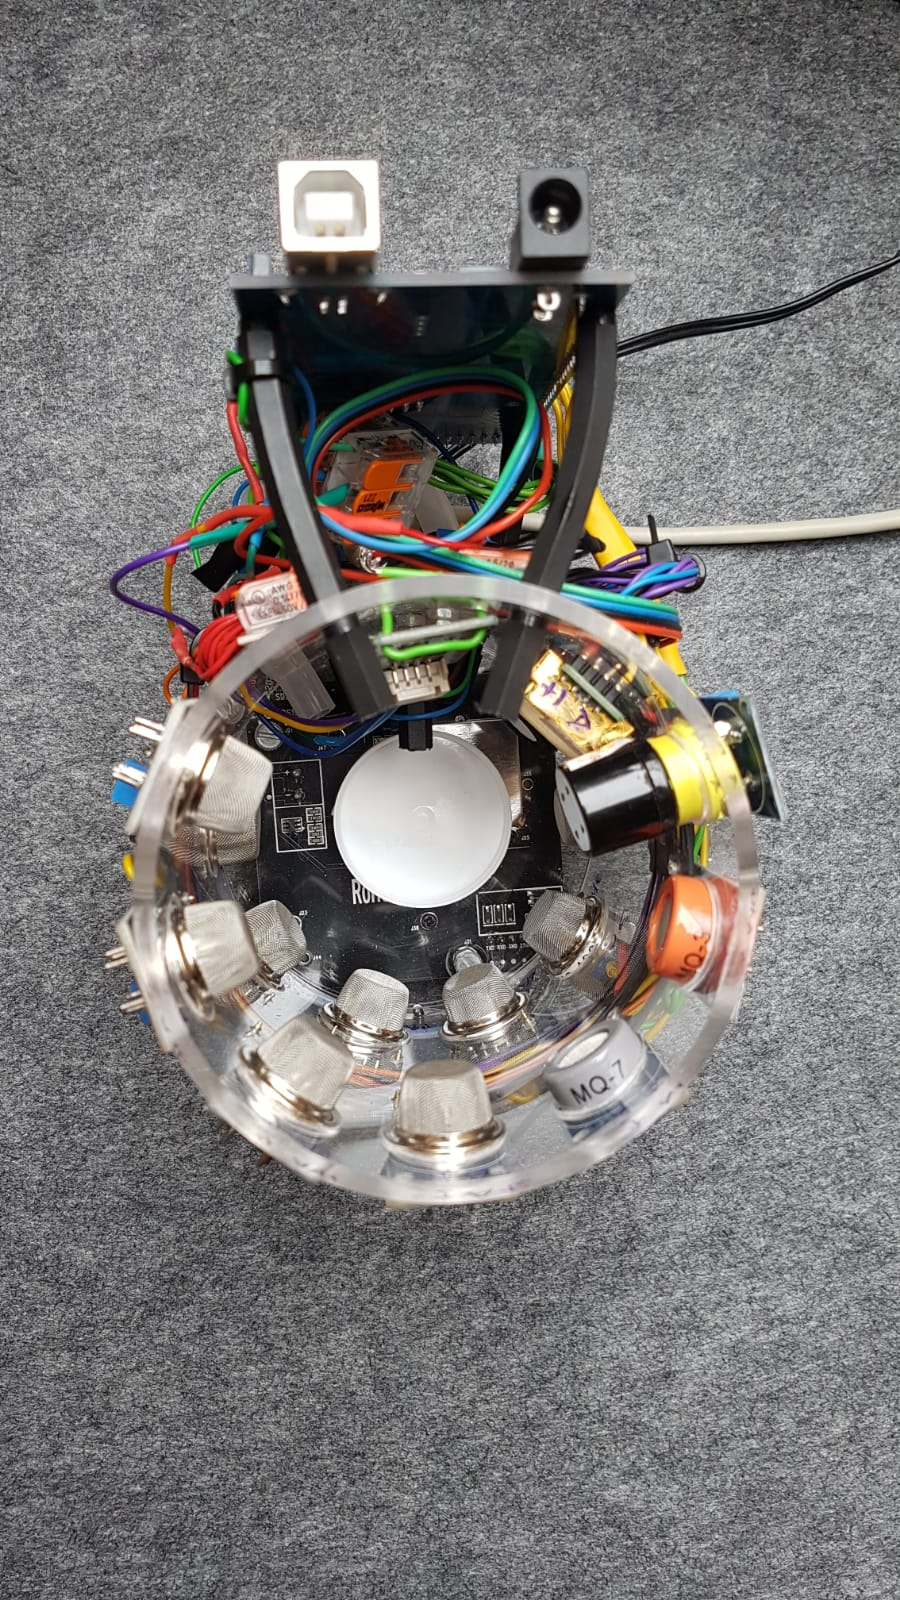
\includegraphics[scale=0.15, angle=90]{Bilder/Nase_Core.jpeg}
\caption{Der Senor-Array}
\label{Nase_Core}
\end{figure} 

Die Abbildung \ref{Nase_Core} zeigt den gebauten Sensor-Array. Das Behältnis ist aus durchsichtigem Acryl, damit man das Innere besser betrachten kann. 
An der Grundfläche des Zylinders ist außerdem ein Auffangbehältnis befestigt, welches
das Messen von Flüssigkeiten ermöglicht. Man kann dieses zum Waschen auch einfach herausnehmen und im Zweifelsfall so dann
auswechseln.\\
Die Sensoren befestigte ich, indem ich Löcher in das Gehäuse bohrte und die Sensoren dann dort einsetze. Um die Befestigung stabiler zu machen,
habe ich die Sensoren außerdem mit Schrauben befestigt. Zwischen Sensor und Rand entstand dabei allerdings jeweils ein
kleiner Spalt (siehe Abbildung \ref{Luecken}), der sich leider kaum vermeiden lässt. 

\begin{figure}[H]
\centering
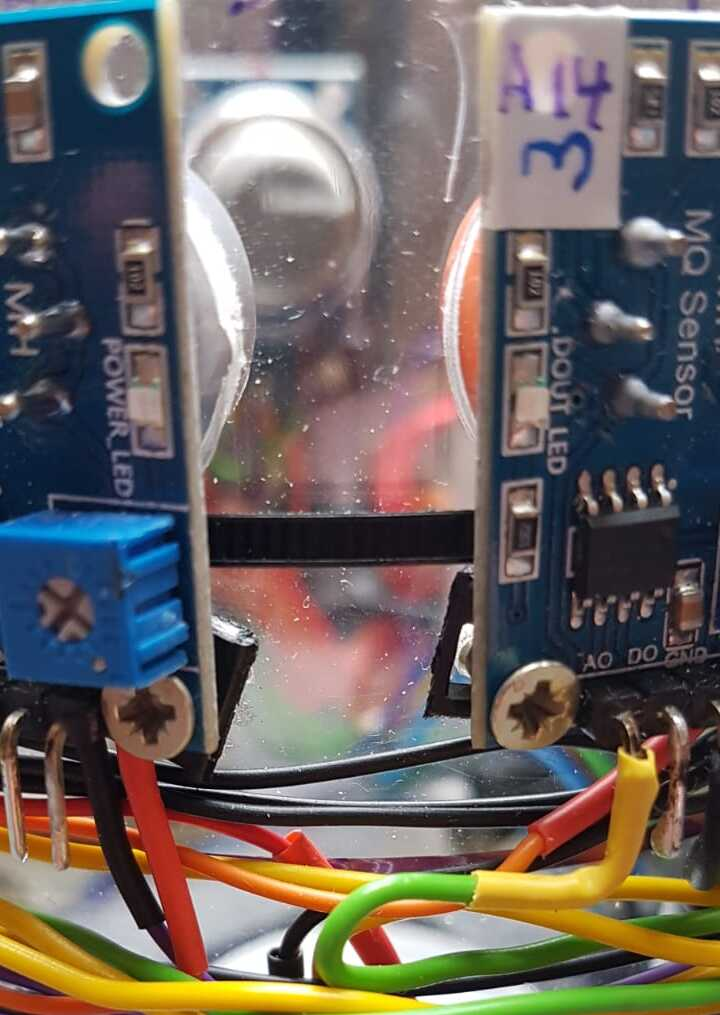
\includegraphics[scale=0.20]{Bilder/Luecken.jpeg}
\caption{Spalt zwischen Sensor und Acryl}
\label{Luecken}
\end{figure} 

Durch diesen könnten Teile des Gases austreten. Ich habe für jenen Fall noch einen zweiten Deckel mit Lüfter, dessen
Luftstrom viel schwächer ist. Dadurch sollte zwar möglichst wenig Gas entweichen, allerdings könnte welches von Außen 
eintreten. Das ist suboptimal, denn ein Austreten des Gases würde die Konzentration im Inneren immer weiter verringern. Man könnte
nun versuchen, die Lücken abzudichten. Das würde sich aber schwierig gestalten. Denn Füllmaterialien wie Silikon oder Knete
haben oft einen eigenen Geruch, welcher die sich direkt daneben befindenden Sensoren beeinflussen könnte. Hinzu kommt, dass das Füllmaterial 
auch zu jeder Zeit dicht sein muss, was bei einem längeren Anwendungszeitraum durch Porosität und gegebenenfalls auch Erschütterungen sehr unwahrscheinlich ist. 
Ich kam deshalb zu dem Entschluss, einfach ein zweites Gehäuse um den Zylinder zu platzieren. Das zweite Gehäuse dient dann
als Abschirmung des Sensor-Arrays von der Umgebung. Das zweite Gehäuse muss keine besonderen Eigenschaften haben, 
aufgrund der Unkompliziertheit baute ich also einfach einen Würfel aus mehreren Acrylscheiben zusammen.\\
Durch diesen Acrylwürfel gehen mehrere Kabel für die Stromversorgung, denn die Sensoren in Verbindung mit den Lüftern brauchen ungefähr 3,2 Ampere, bei einer Spannung
von 5 Volt. Eine Leistung, für die definitiv eine externe Stromquelle nötig ist. Nur wenige Netzteile haben diese, weshalb ich anfangs noch zu einem Labor-Netzteil griff. 
Lediglich durch das falsche Drehen am Spannungsregler
hätten die Sensoren dadurch aber allesamt zerstört werden können. Außerdem sind Labor-Netzteile ziemlich schwer, groß und unhandlich. Ich fand glücklicherweise noch einen USB-HUB, welcher 
genug Ampere liefern konnte und somit jetzt zur Stromversorgung genutzt wird.
Zur weiteren Verkabelung der Sensoren dienten außerdem vorerst gewöhnliche Arduino-Jumper-Kabeln. Die sind allerdings
ziemlich dünn. Somit besteht das Risiko, dass die Isolierung der Kabel wegen des hohen elektrischen Wiederstandes anschmort oder die Kabel ganz durchbrennen. 
Als Leiter habe ich deshalb einen viel dickeren Kupferdraht verwendet, um die Sicherheit auch vollends zu gewährleisten.


\subsection{Interface zwischen Sensorik und Software}
Die von den Sensoren ausgegebenen Daten müssen natürlich anschließend eingelesen werden. Da eine Änderung der Konzentration bei allen Sensoren als
Spannungsänderung ausgegeben wird, benutzte ich dazu einen Arduino. Arduinos sind immerhin die am meisten verwendeten 
Mikrocontroller und für solche Zwecke einfach perfekt geeignet. Der Arduino kann dann die Spannungsänderung über seine analogen Pins
messen und anschließend in Binärzahlen umwandeln. Die analogen Pins haben eine Auflösung von zehn Bits, können also Werte von 0–1023 annehmen. Von der ganzen Arduino-Familie
habe ich mich außerdem für einen Arduino Mega entschieden, denn mit dessen 16 analogen Pins hat er genug Inputs für alle MQ-Sensoren, gleichzeitig aber auch noch viele weitere Schnittstellen 
wie $I^2C$ und serielle Verbindungen. Diese kann ich dann für die anderen Sensoren wie den Sauerstoff, VOC und Feinstaubsensor nehmen.
Für den Kohlenstoffdioxid Sensor sind zudem PWM Pins verfügbar. Die Sensorwerte der MQ-Sensoren lassen sich sehr einfach mit einem analogRead() auslesen, während für die meisten
anderen Sensoren vom jeweiligen Hersteller Bibliotheken bereitgestellt werden. Für die Sensoren brauche ich deshalb fast alle Pins, die digitalen ausgenommen. Man kann die Verkabelung
gut in Abbildung \ref{Arduino_Mega} sehen.

\begin{figure}[H]
\centering
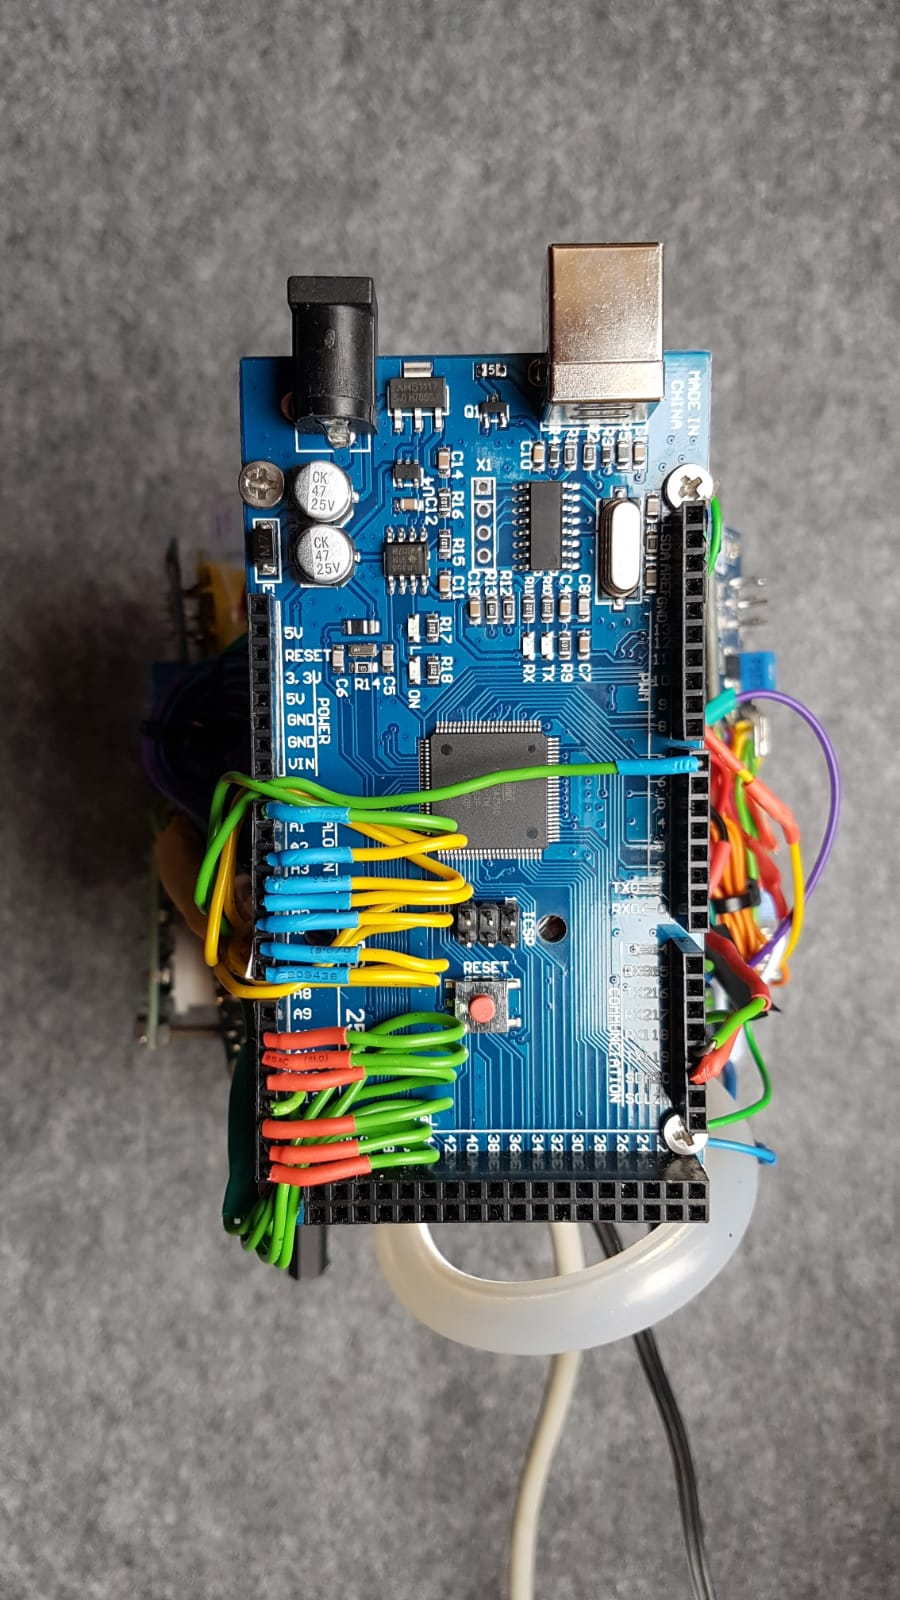
\includegraphics[scale=0.15, angle=90]{Bilder/Arduino_Mega.jpeg}
\caption{Microcontroller}
\label{Arduino_Mega}
\end{figure} 

Der Arduino Mega ist mit einem USB-Kabel an einen PC angeschlossen. Er sendet dann in Windows an dessen COM Port, in Linux an ein character device mounted in /dev,
über den Serial-Bus (UART Schnittstelle) die Sensorwerte. Die von mir programmierte Software kommuniziert dann
über den Port mit dem Arduino. Es werden am Anfang einige wichtige Daten zur Synchronisation ausgetauscht und anschließend sendet nur noch der Arduino
in regelmäßigen Abständen die Messergebnisse. Der Computer dient dabei zur weiteren Verarbeitung. Dafür kann man natürlich jeden normalen Laptop oder PC
verwenden, ich habe mich hier aber für den Rock 4B Plus \autocite{Rock4} entschieden. Das ist ein SBC (Single Board Computer), welcher aufgrund seiner Größe ideal ist.
Die wohl erste Frage wäre wohl: Warum keinen Raspberry Pi? Immerhin haben beide ähnliche Maße. Der Grund dafür ist,
dass die Produktion des Raspberry Pi, zu dem Zeitpunkt, an dem ich diese Arbeit schreibe, vorerst pausiert wurde \autocite{RaspberrySupply}. Vermutlich ist dies auf
die Halbleiter-Krise zurückzuführen. Er ist nun nur noch zu astronomischen Preisen bei wenigen Händlern oder auf Online-Kleinanzeigen-Portalen verfügbar. Selbst 
als gebrauchten Artikel war es mir, obwohl ich Wochen mit dem regelmäßigen Suchen nach einem fairen Angebot eines Raspberry Pi verbrachte, nicht möglich,
einen solchen zu finden.
Der viel weniger bekannte Rock Pi hat dieses Problem momentan (noch) nicht, wodurch er trotz seines etwas höheren Preises
mit vielen weiteren Vorteilen punkten kann: Im Gegensatz zu dem Raspberry Pi besitzt er einen Hexacore, von dem interessanterweise zwei anders getaktet sind
als die restlichen vier. Die CPU des Rock 4B Plus ist also viel leistungsfähiger als die eines Raspberry Pi. Als Betriebssystem bietet der Hersteller "`radxa"'
eine Debian Desktop ISO an. Ich habe diese einfach nach dem ersten Booten von einer $\mu$SD-Karte auf
die integrierte eMMC geflasht. Es gibt zwar auch andere Betriebssysteme, die teilweise von anderen Firmen angeboten werden, Debian erschien mir aufgrund der Stabilität
in diesem Fall aber als am sinnvollsten.\\
Auf dem Linux Betriebssystem konnte ich dann nach der Installation alle nötige Software installieren. Es gibt zwar fast nie eine Version speziell für den Rock 4, aber
für gewöhnlich funktionieren auch die ARM-Versionen, die für einen Raspberry Pi geschrieben wurden. Beispielsweise lassen sich die Processing IDE und die Arduino IDE 
ohne Probleme installieren. Die Processing-Foundation gibt nämlich eine eigene ARM-Version heraus, während die Arduino IDE von einem GitHub 
Nutzer bereitgestellt wird \autocite{ARM_ArduinoIDE}. Zwar ist diese laut der \textit{README.md} auf den Raspberry Pi zugeschnitten, 
auf dem Rock 4B Plus läuft sie aber ebenfalls.\\
Ein weiterer Vorteil eines SBC ist, dass ich ihn aufgrund der geringen Größe mit in das Gehäuse legen kann, ohne dass ich immer einen um ein Vielfaches größeren
PC dabei haben muss. Zudem kann man sich mit diesem über eine ssh (Secure Shell) Verbindung von einem anderen PC aus verbinden (sofern man im gleichen Netzwerk ist). 
Gibt man den ssh Befehl mit der Flag -X oder -Y an, signalisiert man, dass die Fenster des auf dem Rock 4 laufenden x-servers zu dem eigenen PC umgeleitet werden
sollen. Dadurch kann ich auch von meinem Laptop aus 
alle Programme auf dem Rock 4 öffnen und ausführen. Das ist sehr nützlich, um den Arduino zu programmieren, obwohl der Sensor-Array nicht einmal in der Nähe
meines Schreibtisches steht.\\
Doch nicht nur für das Durchführen von Messungen ist der Mini-Computer äußerst hilfreich. Ich verwende ihn auch zur Ausgabe des detektierten Geruchs. Dazu kann ich 
ein kleines 3,5 Inch Display anschließen, welches dann einzig den erkannten Duft anzeigt.
Nach dem Bau des Sensor-Arrays und der richtigen Verkabelung sieht das Ergebnis so aus:\\

\begin{figure}[H]
\centering
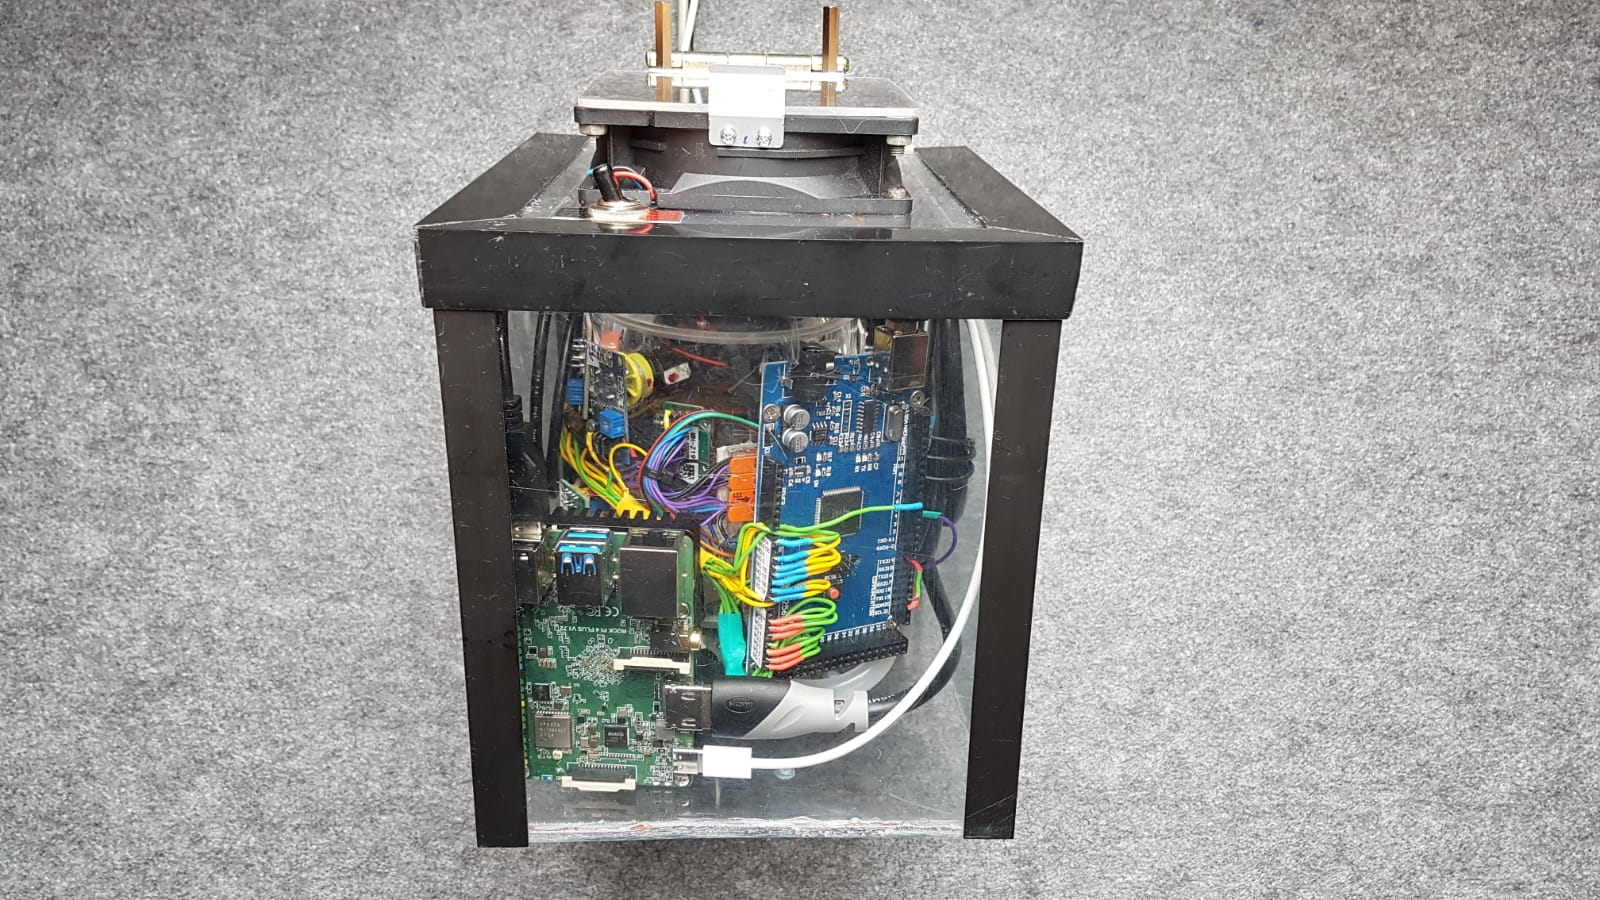
\includegraphics[scale=0.2]{Bilder/Nase.jpeg}
\caption{Sensor-Array mit Ummantelung}
\label{Sensor-Array_mit_Ummantelung}
\end{figure}


\section{Normalisierung der Daten}
Direkt nach dem Bauen der E-Nase testete ich zuerst, ob auch alle Sensoren funktionieren. Anfangs war dies glücklicherweise der Fall, auch wenn sich 
das im Verlauf leider oft änderte und jeweils mehrere Tage zur Fehlerfindung erforderte. Nur bei dem Sauerstoffsensor gibt es einige Ungereimtheiten, denn dort
liegt die gemessene Sauerstoffkonzentration meistens bei ca. 10 \%, was etwas weit von den 21 Prozent in normaler Raumluft entfernt ist.
Wie hoch nun die genaue Konzentration ist, sollte allerdings nicht sehr wichtig sein. Es geht bei der Erkennung schließlich eher um die 
Änderung, als um die tatsächliche Konzentration.\\
Ansonsten waren die Messwerte bei den restlichen Sensoren plausibel. Ich hatte trotzdem einige Bedenken, da die Werte etwas unzuverlässig waren. Es gab immer wieder 
größere Differenzen zwischen aufeinanderfolgenden Messwerten, obwohl sich die Umgebungsluft in keinster Weise änderte. 
Kleine Schwankungen wären zwar normal, jedoch nicht in einem solchen Ausmaß. Die Sensorwerte waren demnach extrem rauschbehaftet,
weshalb eine digitale Signalverarbeitung vor der Erkennung unbedingt nötig war.\\
Dafür gibt es viele Algorithmen, die Abhilfe leisten können. Interessanterweise würde sich zum Beispiel die Fourier-Transformation 
(bzw. die Schnelle Fourier-Transformation) anbieten \autocite{FourierFiltering} \autocite{FourierConvolution}, 
in dem Bereich der Datenverarbeitung wäre es dann speziell die Wavelet-Transformation,
welche auf der Fourier-Transformation basiert \autocite{wavelet}. Doch dies würde das Involvieren von vielen komplexen (im wahrsten Sinne des Wortes) Vorgängen bedeuten.
Damit ist eine solche Methode immer noch etwas weit von einer sehr effizienten Lösung entfernt. Für viel interessanter fand ich daher das Prinzip der 
Sensor-Fusion \autocite{SensorFusionAndKalmanFilter}.
Dabei misst man ein Gas mit mehreren (allesamt unzuverlässigen) Sensoren und kombiniert die erhaltenen Werte anschließend zu einem einzigen, sehr viel weniger
rauschbehafteten, Sensorwert. Das Kombinieren der Sensorwerte kann dann beispielsweise mit einem Kalman-Filter \autocite{SensorFusionAndKalmanFilter} ermöglicht werden. Nun ist es aber so, dass
ich nicht von jedem Sensor mehrere kaufen möchte. Das würde das Gehäuse riesig machen und zudem eine immense Herausforderung an den Arduino Mega stellen, ganz zu schweigen davon, dass
dieser nicht einmal so viele analoge Pins hätte. Ich habe deshalb einen für mich viel simpleren Ansatz der Sensor-Fusion genommen. Anstatt pro Messung mehrere Sensorwerte
zu erhalten, kombiniere ich einfach einige aufeinanderfolgende Messungen. Somit kann ich die Messwerte zusammenfassen und dann glätten, zum Beispiel mit der Berechnung des gleitenden Mittelwerts
oder des exponentiellen Mittelwerts. Um auch wirklich qualitative Messwerte zu erhalten, finde ich aber die Berechnung eines einzigen Mittelwerts  sinnvoller. Um das Prinzip in der Praxis zu testen, 
unternahm ich ein paar Versuche. Ich stellte fest, dass der Durchschnitt von ungefähr 50 (!) Sensorwerten berechnet werden muss. Und das
pro Sensor. Das ist aber akzeptabel, denn einige Sensoren (insbesondere die $I^2C$ Sensoren) haben Bibliotheken, die jeweils ähnliche 
Berechnungen anstellen \autocite{SGP40Library}. Im Allgemeinen lässt sich sogar sagen, dass sich die bereitgestellten Bibliotheken nur an den Sensorwerten orientieren. Vor der wirklichen
Ausgabe des jeweiligen Sensorwerts werden noch viele Berechnungen angestellt, die die Messergebnisse verbessern. Jedenfalls entnehme ich das so aus dem jeweils verlinkten Source-Code.\\
Durch das Berechnen des Durchschnitts sieht der Graph von normaler Luft nun so wie in Abbildung \ref{Ergebnis der Durchschnitsberechnung} aus:\\

\begin{figure}[H]
\centering
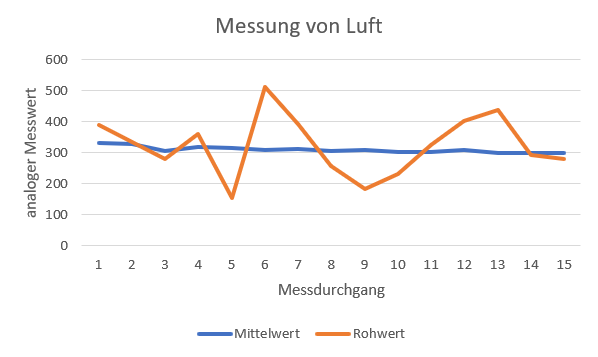
\includegraphics[scale=0.8]{Bilder/Messung_von_Luft.png}
\caption{Ergebnis der Durchschnitsberechnung}
\label{Ergebnis der Durchschnitsberechnung}
\end{figure} 

Die Messwerte sind bereits durch diese Änderung sehr viel stabiler. Man darf aber nicht vergessen, dass sie die absolute Konzentration abbilden.
Das bedeutet, dass die Messergebnisse schon vor der Messung von der Umgebungsluft beeinflusst werden. Denn jede Raumluft ist in ihrer Zusammensetzung etwas anders. Das fängt schon damit an, wann
das letzte Mal gelüftet wurde. Es ist deshalb weitaus sinnvoller, den Algorithmen nicht die absolute Konzentration betrachten zu lassen, sondern die Differenz zwischen dem betrachteten
Wert und der "`normalen"' Umgebungsluft. Dazu habe ich am Anfang jeder Messung eine "`Kalibrierungsphase"' eingerichtet. In dieser Phase wird mehrmals gemessen, was für jeden Sensor
der normale Wert in Raumluft ist, ganz ohne zu erkennenden Geruch. Dieser Wert kann dann anschließend während der Messung jedes Mal von dem tatsächlich beobachteten Wert abgezogen werden. 
Ich messe damit also nicht die wirkliche Konzentration, sondern nur die Änderung zum (am Anfang gemessenen) Normalwert. Deshalb auch Kalibrierungsphase, die Sensoren werden auf die Raumluft 
kalibriert.\\
Durch die Kalibrierungsphase sind die Sensorwerte in der Raumluft (aufgrund der Berechnung der Differenz) alle ungefähr auf null, natürlich mit Schwankungen. Dies ändert sich dann
erst durch das Einlassen eines zu messenden Gases. Was den Einfluss des Geruchs auf die Sensorwerte betrifft, nehme ich Folgendes an:\\
\\
Es gibt eine Menge an Sensorwerten, die der Sensor-Array ausgeben kann. Ich nenne diese $W$, wie Wertebereich.
Die Menge der Sensorwerte, welche ein Geruch verändert/beeinträchtigt, heißt $B$, wie beeinträchtigt.
Logischerweise ist nun $B$ eine Teilmenge von $W$, also $B \subset W$.
$B$ kann somit auch synonym mit dem Begriff Geruch verwendet werden, da diese Menge den Geruch überhaupt erst charakterisiert.
Es lässt sich nun also jedem von der Messtechnik erfassbaren Geruch $g$ eine Menge $B_g$ zuordnen, welche deshalb auch als Geruchsprofil von $g$ bezeichnet werden
kann, denn sie profiliert $g$ eindeutig. Die Ausnahme bildet der Sonderfall $B = \emptyset$, wobei der Geruch aufgrund der Grenzen der Messtechnik nicht erkennbar ist.
Mit der (nicht leeren) Menge $B_g$ sollte es also möglich sein, den Geruch $g$ eindeutig zu erkennen und von anderen Gerüchen zu unterscheiden. 
Eine Abgrenzung zwischen verschiedenen Gerüchen funktioniert allerdings nur, wenn es kein Geruchsprofil gibt, was dem eines beliebigen anderen Geruchs $x$ gleich ist, 
also $\neg \exists g (B_g = B_x)$ \\
Außerdem treffe ich die Annahme, dass das Größenverhältnis der Elemente von $B$ sich nicht mit der Zunahme der Konzentration des Gases ändert. Nimmt die Konzentration des Gases zu, ändern sich also
alle Sensorwerte $s \in B$ proportional zur Zunahme der Konzentration $p$ ( $\forall s \in B : s \propto p$).\\
\\
Nachdem ich diese Erwartungen/Annahmen getroffen hatte, fiel mir ein Problem auf:
Den Gerüchen ist auf diese Art und Weise nicht immer ein einzigartiges Profil zuzuordnen. Jedenfalls nicht aus der Sicht der Software. Denn momentan ändert sich das Geruchsprofil
je nach Konzentration, also der Intensität des Geruchs. Vielleicht wäre das in der Zukunft gut, falls ich dann auch die Intensität bestimmen möchte. Momentan reicht aber die
erfolgreiche Bestimmung des Geruchstyps, wofür jene Information irrelevant ist. Eine Lösung fand ich aus dem Bereich des Machine Learnings. Denn zumindest von dort kenne ich die sogenannte "`Softmax Funktion"', welche sich äußerster Beliebtheit erfreuen kann. Sie ist wie folgt definiert:
$$ \sigma (\mathbf {z} )_{j}={\frac {e^{z_{j}}}{\sum _{k=1}^{K}e^{z_{k}}}}$$
Die Funktion ist aus mehreren Gründen beliebt. Einer wäre, dass sie die Werte des Ausgabevektors zwischen Null und Eins begrenzt. In diesem Fall benutze ich sie
aber, da sich die Ausgabewerte zu Eins aufsummieren. Die Werte stehen dabei alle in Relation zueinander. Der Ausgabewert $y_i$ kann also
als Prozentsatz angesehen werden, wie hoch das zugehörige (korrespondierende) $x_i$ relativ zu den anderen x-Werten ist. Analysieren die Algorithmen also nur
die y-Werte, macht es am Ende keinen Unterschied, wie hoch die Konzentration ist! Die Werte der Softmax-Funktion ändern sich in dem Fall nicht. Denn da ich erwarte, dass 
die Sensorwerte proportional mit der Konzentration zunehmen, kann sich der Output der Softmax Funktion bei gleichem Gas und unterschiedlicher Konzentration nicht verändern.\\
Als kleine Zusammenfassung: Die Sensorwerte werden fünfzigmal eingelesen. Aus diesen Messwerten wird dann der Durchschnitt berechnet, welcher anschließend an den Rock 4 geschickt wird.
Dort wird nach dem Empfangen eines "`Datasets"', also einer vollständigen Menge $W$, aus den Werten das Ergebnis der Softmax-Funktion berechnet. Diese Werte können dann mit Algorithmen 
der Mustererkennung weiter analysiert werden. Bei dem Ablauf fehlt nur ein Schritt, den ich bis jetzt noch nicht beachtete: Bevor die Sensorwerte durch die Softmax Funktion laufen,
sollten sie am besten die gleiche Einheit haben. Denn ansonsten tritt das Problem auf, dass die Ausgabewerte ziemlich klein werden. Ein Beispiel: In Raumluft
gibt es einige MQ-Sensoren, die einen Wert von ungefähr 600 ausgeben. Während der gleichen Messung hat der VOC Sensor aber Werte, die kleiner als 100 sind. Der von der Softmax ausgegebene
prozentuale Wert wäre nun im Fall des VOC Sensors extrem klein, vermutlich mit sehr vielen Nachkommastellen. Sofern man dies mathematisch betrachtet, ist das nicht weiter schlimm. 
In der Informatik ergibt sich aber die Problematik, dass Zahlenwerte nun nicht unendlich groß oder klein sein können. Es würde durch die Begrenzung der Nachkommastellen von zum Beispiel eines Doubles oder selbst eines "`BigDecimal"' Objekts ein Großteil der Präzision verloren gehen. Deshalb ist es sinnvoll, die Zahlen vorher in einen gleichen Wertebereich zu überführen. 
Eine Möglichkeit wäre die Umrechnung in dieselbe Einheit gewesen. Hier hätte sich ppm angeboten, was für parts per million steht (x ppm == x Moleküle in einer Million Moleküle).
Der von den Sensoren ausgelesene Wert gibt aber die anliegende Spannung an. Es gibt deshalb Formeln, mit denen man die Einheiten ineinander umrechnen kann \autocite{MQToPPM}. Selbst auf
diese Weise wäre die Verteilung allerdings immer noch viel zu unterschiedlich. Denn allein der Sauerstoffsensor gibt in meiner Raumluft ungefähr 10 Prozent aus,
was 100 000 ppm wären. Würde er die korrekten 21 Prozent anzeigen, wären es natürlich dementsprechend mehr. Der Unterschied zu den anderen Sensorwerten wäre hier womöglich noch größer als zuvor. 
Deshalb möchte ich das Problem durch das Skalieren der Werte lösen.
Die Formel dafür würde im Quellcode so lauten:\\
$$ wert_{t} = min_{t} + (max_{t} - min_{t}) * ((wert_{t-1} - min_{t-1}) / (max_{t-1} - min_{t-1}))$$
$wert_{t-1}$ ist der alte, zu verändernde Wert. $min_{t-1}$ ist dann das alte Minimum und $max_{t-1}$ das alte Maximum. Die neuen Werte, also die nach der Transformation, 
sind dann dementsprechend die mit $t$ als Index. Die Formel möchte ich dafür benutzen, um alle Werte auf ein neues Minimum von 0 und neues Maximum von 1 zu skalieren.
Bei allen Sensoren wäre das alte Minimum dann 0. Aber was sollte das alte Maximum des jeweiligen Sensors sein? Zuerst dachte ich, man könnte einfach
den im jeweiligen Datenblatt genannten maximalen Ausgabewert benutzen. Im Falle der MQ-Sensoren, die analoge Messwerte liefern, wäre das 1023 gewesen (denn 10 Bits).
Bei den anderen Sensoren unterscheidet sich das aber stark.
So zum Beispiel der Feinstaubsensor, der laut Datenblatt ein Maximum von $1000 \frac{\mu g}{m^3}$ aufweist \autocite{Staubsensor}. Der Wert ist aber sehr weit von den 
tatsächlichen Messungen entfernt, die selten größer als  $10 \frac{\mu g}{m^3}$ wurden. Den angegebenen Maximalwert würde ich damit also nie auch nur im Entferntesten erreichen, 
was die Werte weiterhin nicht wirklich vergleichbar machen würde.\\
Schlussendlich setzte ich dann folgende Lösung um: Als jeweiliges altes Maximum betrachte ich nun einfach den größten Wert, den ich mit dem jeweiligen Sensor jemals gemessen habe.
Dieser Maximalwert kann sich natürlich dauernd ändern, dessen Dynamik ist aber nicht weiter hinderlich. Denn das ändert immerhin nicht den Output der Softmax Funktion.
Bevor die Softmax Funktion also angewandt wird, werden die Messwerte wie folgt skaliert:
$$ wert_{t} = min_{t} + (max_{t} - min_{t}) * \frac{wert_{t-1} - min_{t-1}}{max_{t-1} - min_{t-1}}$$
%$$ wert_{t} = 0 + (max_{t} - 0) * \frac{wert_{t-1} - 0}{max_{t-1} - 0}$$ % unnötig zu schreiben
$$ wert_{t} = \frac{wert_{t-1} }{max_{t-1}}$$

\newpage

\section{Die Messungen}
Bevor ich mit einer Messung beginne, gebe ich den Sensoren Zeit, um sich aufzuwärmen.
Denn in den Datenblättern ist jeweils eine Vorheitzzeit angegeben, die bessere Sensorwerte verspricht.
Diese ist aber bei allen Sensoren unterschiedlich hoch und kann von wenigen Sekunden bis hin zu mehreren Tagen reichen.
Deshalb habe ich mich für eine, nicht sehr genau einzuhaltende, Vorheizzeit von etwa einer Minute entschieden. In den 60 Sekunden
sollten sich alle Sensoren weitestgehend aufgewärmt haben und da ich keine besonders genauen Messwerte brauche, sollte das reichen.\\
Nach der Vorheitzzeit beginnt die Kalibrierungsphase. Wie bereits erwähnt, stellt sich hier die Software auf die neue Raumluft ein.
Zwar lüfte ich das gesamte Gehäuse nach einer jeden Messung mithilfe der Ventilatoren, trotzdem kalibriere ich die Software vorsichtshalber
nach jeder Messung erneut. Nach der Kalibrierung kann ich dann den zu messenden Stoff in den Zylinder des Sensor-Arrays legen,
alles verschließen und die Messung starten. Während des Messvorgangs werden von der Software die derzeitigen Messwerte visualisiert. Das ist vor allem hilfreich, da man so gleich erkennen
kann, ob man die Messung beispielsweise zu früh gestartet hat. Wäre der Deckel zum Beginn der Messung noch offen, würde das nämlich sehr wahrscheinlich die Messwerte beeinflussen.
Etwas Derartiges macht sich dann auch in den Diagrammen bemerkbar. Neben der grafischen Darstellung, welche auf eventuelle Fehler hinweisen kann, gibt es dann noch ein Control Panel, welches dem 
Starten/Stoppen von Messungen, aber auch dem Hinzufügen neuer Geruchsnamen dient. Schlussendlich wird das Ergebnis der Algorithmen, die den Geruch klassifizieren, in einem vierten und letzten
Fenster angezeigt. Wird keine Messung genommen, wird die Software automatisch im Debug-Mode gestartet. Dabei wird im Balkendiagramm einfach eine der letzten Messungen angezeigt und
in dem Liniendiagramm der Verlauf aller Messungen, die jemals genommen wurden. Als Erkennungsergebnis wird zudem einfach nur ein Fragezeichen dargestellt. 
Das sieht dann beispielsweise so wie in Abbildung \ref{Messungs-Software} aus:

\begin{figure}[H]
\centering
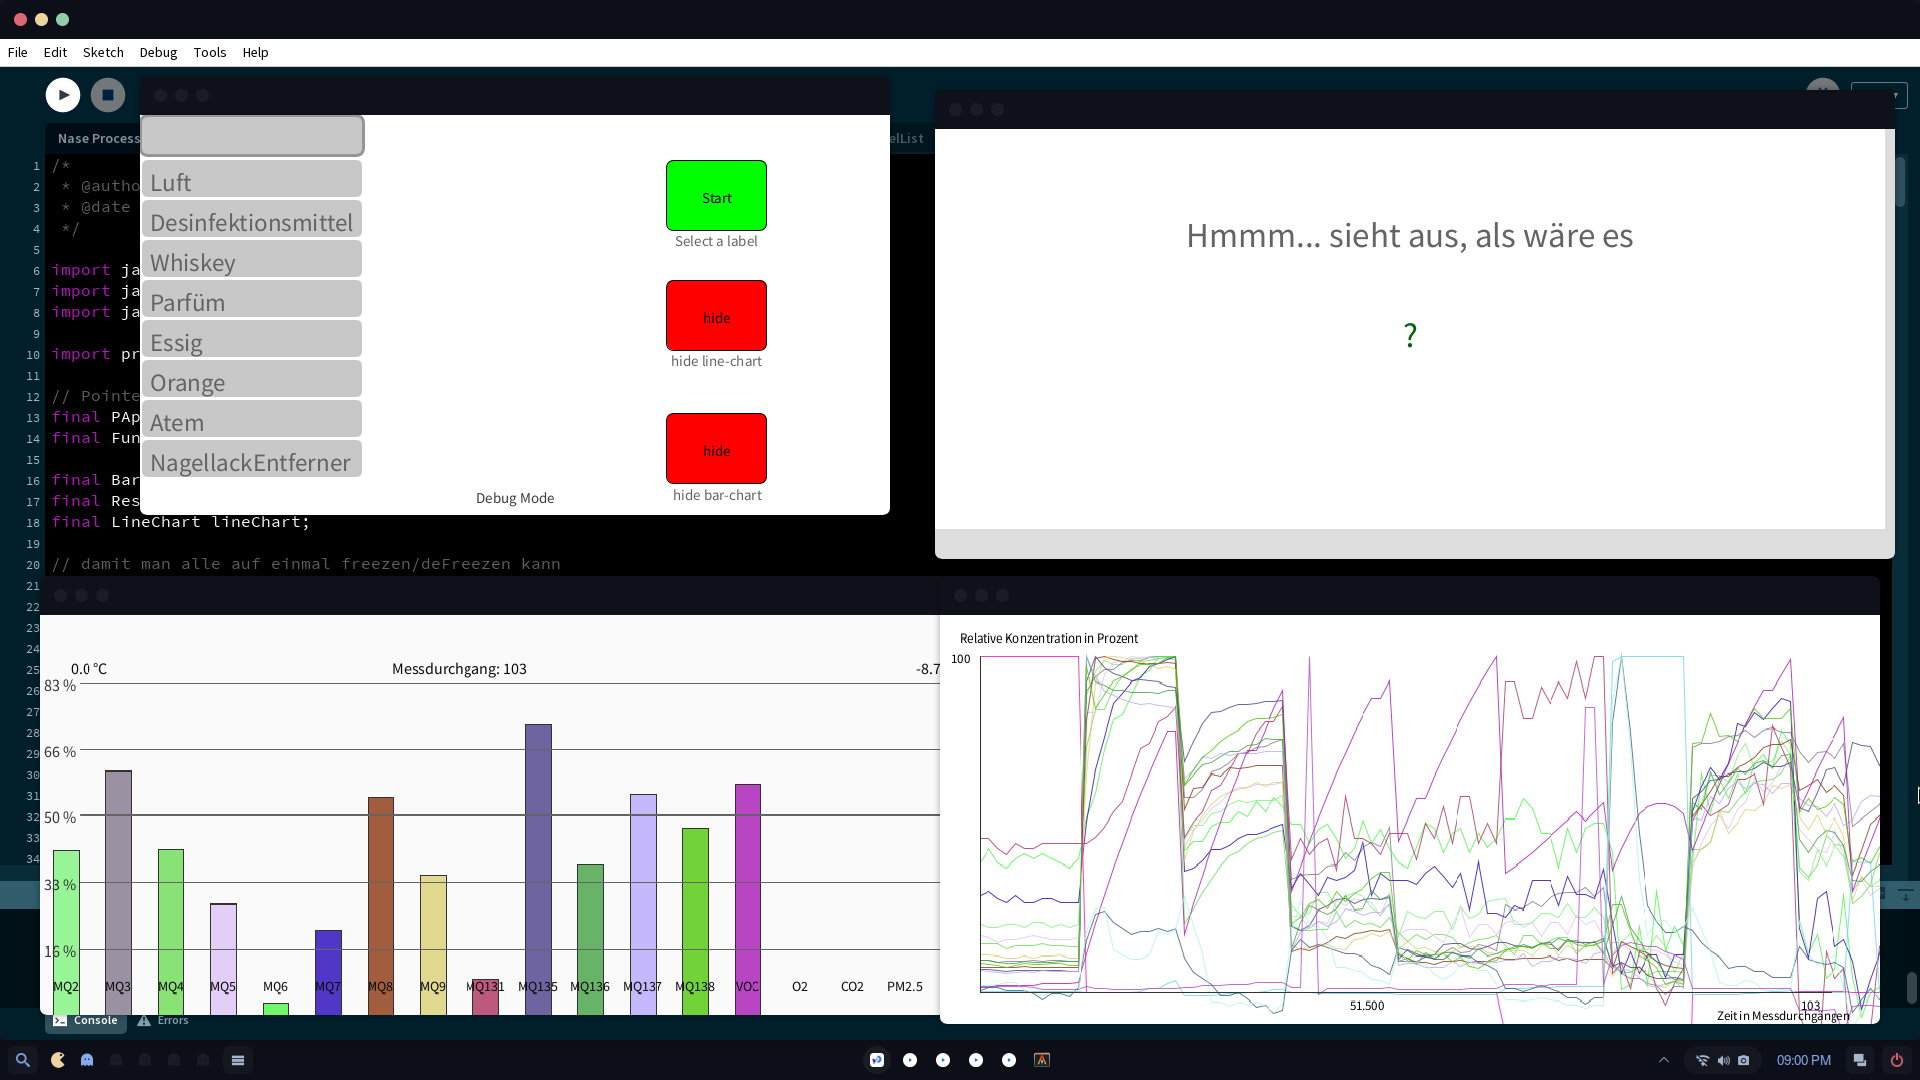
\includegraphics[scale=0.25]{Bilder/MessungsSoftware.png}
\caption{Die Messungs-Software}
\label{Messungs-Software}
\end{figure}

Stoppt man die Messung mithilfe des Control-Panels, werden alle gesammelten Messwerte gespeichert. Sollte eine neue Geruchsart hinzugekommen sein, würd dies ebenfalls gesichert. 
Mit der Zeit kommt dabei allerdings eine beträchtliche Menge an Sensorwerten an, die auch viel Speicherplatz benötigt. Damit die Dateigröße möglichst klein bleibt,
habe ich deshalb einen Algorithmus programmiert, der die Werte eines (multidimensionalen) Java-Arrays binär speichert. Der in der Datei gespeicherte Array kann dann
anschließend wieder geladen werden, damit die Mustererkennung die Beispiele zum Training verwenden kann.

\subsection{Verarbeitung}
Ich möchte mich in dieser Arbeit primär auf die mathematische und technische Umsetzung konzentrieren. Es sei aber gesagt,
dass der wohl mindestens genauso große Aufwand bei dem Schreiben der Software entstand – insbesondere natürlich dem Debuggen. 
Und dabei möchte ich nicht einmal an die unzähligen Probleme denken, die ich mit der Hardware hatte.\\
Das Thematisieren des Codes finde ich aber ziemlich sinnlos, denn dafür gibt es immerhin Kommentare. Und das Einfügen meines Source Codes ist schließlich auch
nicht die Idee hinter einer schriftlichen Arbeit. Ich würde mich also sehr freuen, wenn Sie sich vielleicht auch noch die Zeit nehmen würden, sich zumindest Teile des Quelltextes anzusehen.
Ich habe dabei die beiden Programmiersprachen Java und Python verwendet. Der Code findet sich in einem Git-Repository unter \url{www.github.com/JakobZoephel/}.
Außerdem sind dort einige andere Dokumente zu finden, beispielsweise die \textit{.tex} Datei dieser Arbeit.\\
Es ist vielleicht auch wichtig zu wissen, dass die Messungs-Software mit Processing geschrieben wurde. Dies ist prinzipiell ein Software-Projekt 
für Designer und Grafiker, die Animationen und ähnliches mit Java erstellen wollen. Es war vor vielen Jahren
mein Einstieg in die Programmierung, setzt mir heutzutage aber einige Grenzen, zum Beispiel sind alle Variablen sehr Python-ähnlich per default public, was sich nicht ändern lässt
(Grund ist, dass alle definierten Klassen automatisch nested sind und derselben Superclass angehören). 
Da mir die Software dafür sehr vertraut ist, habe ich es auch noch dieses Mal zu der einfachen
Erstellung der GUI benutzt. Alternativen wären natürlich das .NET Framework, GTK+ oder Qt gewesen. Davon ist ersteres für mich als Arch Linux Benutzer etwas suboptimal, während ich mit
den beiden anderen noch nicht genügend Erfahrung habe. Die nun also mit Processing geschriebene Messungs-Software übernimmt also prinzipiell die Aufgabe des einfachen Durchführens von Messungen, 
wobei dies mithilfe der GUI erleichtert wird. Somit ist auch Laien das Messen von Gerüchen möglich. Das Konzept ist dahingehend, dass ich in die Software
zwar bereits einige Beispielgerüche einprogrammiert habe, diese aber bei weitem nicht alle Möglichkeiten abdecken. Man kann vielmehr seine eigenen Gerüche nach und nach selber hinzufügen. 
Somit ist es jedem möglich, das erkennbare Geruchsspektrum für eigene Stoffe und Bedürfnisse leicht anzupassen.\\
Während die Messungs-Software also in Java geschrieben ist, habe ich für das Trainieren der KI, das Erstellen einiger Diagramme und anderer Verarbeitungsschritte Python genutzt.
Der Python Code trägt also nicht direkt zum Funktionsumfang der Messungs-Software bei, ich verwende ihn zu größten Teilen zu Testzwecken. Dazu benutze ich Bibliotheken
wie TensorFlow, NumPy, Keras-Tuner, Scikit-Learn und Matplotlib, um mithilfe von Data Science die bestehenden Funktionen zu verbessern.


\subsection{Mustererkennung}
Aus den gesammelten und vorverarbeiteten Daten muss der Geruchstyp identifiziert werden. Es sind also Algorithmen nötig, die aus den Daten
Geruchsprofile herauslesen und anschließend interpretieren können. Am einfachsten wären dabei aus meiner Perspektive ein sogenannte Decision Tree oder sogar ein Random Forest. 
Das sind, stark heruntergebrochen, im Wesentlichen viele aufeinander folgende if-Abfragen, welche die Daten anhand der Überschreitung von zuvor gelernten Schwellwerten einteilt. 
Meine Intuition war dabei, dass das Ansteigen von bestimmten Sensorwerten automatisch mit einem Geruch verknüpfbar ist. Es stellt sich hier aber ein Problem heraus: Wie bereits erwähnt, 
sind die Messwerte von großen Fluktuationen beeinträchtigt. Zwar habe ich der Beseitigung von diesen schon einen gesamten Abschnitt gewidmet, allerdings sind sie immer noch spürbar.
Der Sachverhalt wird sehr gut von dem Balkendiagramm in der Messungs-Software visualisiert. Dieses wird nämlich jedes Mal aktualisiert, wenn neue Sensorwerte empfangen werden.
Dabei fällt auf, dass sich die Messwerte stetig ohne erkennbaren Grund ändern. Das ist anhand der Balken mit bloßem Auge deutlich zu erkennen. Die Werte ändern sich, obwohl in der Umgebungsluft
keine Änderung erfolgt sein müsste. Es gab nun also die Möglichkeit, die Daten noch weiter zu bearbeiten. Allerdings habe ich dort bereits das offensichtlichste getan,
weshalb weitere Verfahren ziemlich komplex werden könnten. Damit wäre auch einiges an Rechenzeit verbunden, da die grundlegende Bereinigung von Daten von dem leistungsschwachen
Arduino übernommen werden muss. Denn das Senden von solch vielen Rohdaten zu dem Computer würde eine sehr große Latenz einführen, wodurch es sich nicht lohnen würde.
Der Arduino muss schon mit der derzeitigen Konfiguration 150 Millisekunden warten, bevor er die Daten über den Serial-Bus schickt. Bei einer geringeren Pause gehen 
ansonsten zwischendurch Messwerte verloren. Deshalb dauert ein Messdurchgang,
in dem von jedem Sensor ein Wert berechnet wird, bereits mehrere Sekunden. Durch diese Trägheit würde die Erkennung mit der Einführung weiterer
Techniken nochmals länger dauern, als sie es ohne hin schon tut.\\
Ich versuchte also, zu fortgeschrittenen Mittel zu greifen. Eine Idee war zuerst das alternative Nutzen von SVMs, kurz für Support Vector Machines.
Das hört sich etwas kompliziert an, bedeutet aber prinzipiell genau eines:
Man versucht, die Trainingsdaten so gut es geht in Gruppen aufzuteilen, denen man dann die zu untersuchenden Gerüche zuordnen kann. Aber zum ersten ist
hier das Training sogenannter "`Hyperplanes"' notwendig. Außerdem funktionieren SVMs nur, wenn die Daten linear trennbar sind.
Deshalb wäre vermutlich noch weitere Vorverarbeitung wie Kernel-PCA notwendig, was aber auch keine garantierte Erfolgschance verspricht. Dessen Ergebnis hängt
nämlich von den Eigenvektoren des Trainingsdatensatzes ab. Etwas besser finde ich den k-neighrest-neighbor Algorithmus, kurz KNN. Wenn ich einen neuen Geruch aufnehme, wird dann einfach berechnet, 
welcher der von mir bereits klassifizierten Gerüche diesem am ähnlichsten ist. Es wird also einfach von $k$ Objekten der euklidische oder Manhattan-Metrik Abstand
zu dem Geruch berechnet. Die Klasse, die in meinen $k$ nächsten Objekten am meisten vertreten war, ist dann das Ergebnis. $k$ muss für eine eindeutige 
Schlussfolgerung natürlich ein Vielfaches der verfügbaren Klassen plus eins sein, da es sonst zu einem Unentschieden kommen könnte. Der KNN Algorithmus hätte aber sehr wahrscheinlich Probleme
damit, dass die Fluktuationen in den Messwerten ziemlich willkürlich sind. Er könnte also nie einen exakt passenden Geruch finden, da jedes Mal eine zufällige Änderung die Messwerte
in unterschiedliche Richtungen verändert. Es bestünde nun die Möglichkeit, mithilfe von Reinforcement Learning die Daten vorher zu bereinigen. Hier würde ich auch keine Trainingsdaten brauchen,
allerdings hege ich die Sorge, dass das Model zu eifrig werden würde. Damit meine ich, dass es in den meisten Fällen anstatt die Daten zu bereinigen, eher echte Datenvarianz unterdrücken könnte. 
Wegen dieses Dilemmas nutze ich nun einen anderen Typ von Künstliche Intelligenz, und zwar ein Neuronales Netz. Dieses bekommt die verschiedenen Sensorwerte als Eingabe und soll anhand von
diesen bestimmen, welcher Geruch vorliegt. Die Aufgabe der KI ist dann zusätzlich, auch mit dem restlichen Rauschen in den Daten zu handhaben.\\
Üblicherweise benutzt man für das Training von KIs Machine Learning Bibliotheken. Ich habe TensorFlow benutzt, was neben PyTorch wohl das verbreitetste
Tool in diesem Bereich ist. Ich habe dann also die Trainingsbeispiele, welche ich in Processing mit der Messungs-Software erstellt hatte, in Python geladen und anschließend
mit TensorFlow ein selbst definiertes Model trainiert. Der Python Code dazu ist ebenfalls auf GitHub zu finden. Man kann nun das Python-Script mit den erforderlichen Inputs aufrufen, wobei
der Output dann einfach nach std::out geschrieben wird. Alternativ könnte man das trainierte Model aber auch in "`TensorFlow for Java"' \autocite{TFJava} laden, wobei der
Python-Interpreter überflüssig werden würde.\\
Nach dem Trainieren erhielt ich auf dem KNN Algorithmus eine Genauigkeit von neunzig Prozent, während bei dem Neuronalen Netz
alle Testbeispiele korrekt klassifiziert werden konnten.

\section{Ergebnisdiskussion}
Nach mehreren Messungen und einigem Training der Algorithmen können mittlerweile viele Gerüche erfolgreich erkannt werden.
Dazu zählen Luft, Atem, Orange, Desinfektionsmittel, Essig, Nagellack-Entferner, Whiskey und Parfüm. \\
"`Luft"' bezeichnet dabei den Zustand, in 
dem kein Geruch vorhanden ist – denn auch solch einfach Dinge muss ein Computer lernen. Wie bereits erwähnt, dienen diese Gerüche erstmal nur als Basis für weitere, 
den Anwendungsfällen entsprechenden Anwendungen. Die Gerüche wurden ohne ein bestimmtes Muster gewählt, sie waren lediglich einfach in meinem Haushalt zu finden.\\
Die Software kann also alle von den Sensoren erfassbaren Gerüchen erkennen. Wichtig ist, dass es nun einmal auch wirklich nur die von der Messtechnik
erfassbaren sind. Beispielsweise war es mir nicht möglich Knoblauch, Zwiebeln oder Pfeffer erkennen zu lassen. Diese Gerüche enthalten anscheinend Duftstoffe, welche entweder zu gering
in ihrer Ausprägung sind oder nicht von den verwendeten Sensoren wahrgenommen werden können. Um trotzdem zu prüfen, wie maßgeblich die verschiedenen
Sensoren jeweils an der Erkennung beteiligt sind, habe ich das Prinzip der Hauptkomponentenanalyse angewandt.
Die englische Abkürzung ist PCA, was für Principal Component Analysis steht. Ich kann damit berechnen, für wie viel Varianz die jeweiligen Sensorwerte in den Daten sorgen.
Das genaue Ergebnis der PCA findet sich im Zusatz \ref{PCA}. Interessant ist, dass der Kohlenstoffdioxid-Sensor und der Feinstaubsensor zusammen fast 95 Prozent ausmachen!
Das bedeutet aber nicht, dass man mit diesen beiden Sensoren dann auch 95 Prozent der Gerüche erkennen würde. Man kann es ungefähr so sehen: Wenn bei dem $CO_2$ Sensor eine
Änderung auftritt, dann ist diese normalerweise gleichzeitig ziemlich groß. Das Gleiche gilt für den Feinstaubsensor. Die anderen Sensoren sind in ihrer Sensibilität etwas sanfter,
weshalb sich deren Sensorwerte in einem viel kleineren Maßstab ändern. Die PCA funktioniert nun mathematisch so, dass sie große Änderung als Hauptkomponenten bevorzugt.
Die PCA ist damit also aufgrund der schwierigen Vergleichbarkeit der Sensorwerte nicht als extrem genau zu betrachten. Trotzdem kann man anhand der Werte
grob schlussfolgern, dass bei weitem nicht alle Sensoren an der Erkennung beteiligt sind. Fairerweise sei gesagt, dass ich für solche Sensoren erkennbare Gase noch nicht gemessen habe.
Falls ich dann doch einmal an zum Beispiel Methan, Kohlenmonoxid oder ähnliches komme, würde die Verteilung vermutlich anders aussehen.
Dennoch lassen sich die verschiedenen Gruppenzugehörigkeiten der Messdaten schon anhand der ersten drei Hauptkomponenten gut veranschaulichen:

\begin{figure}[H]
\centering
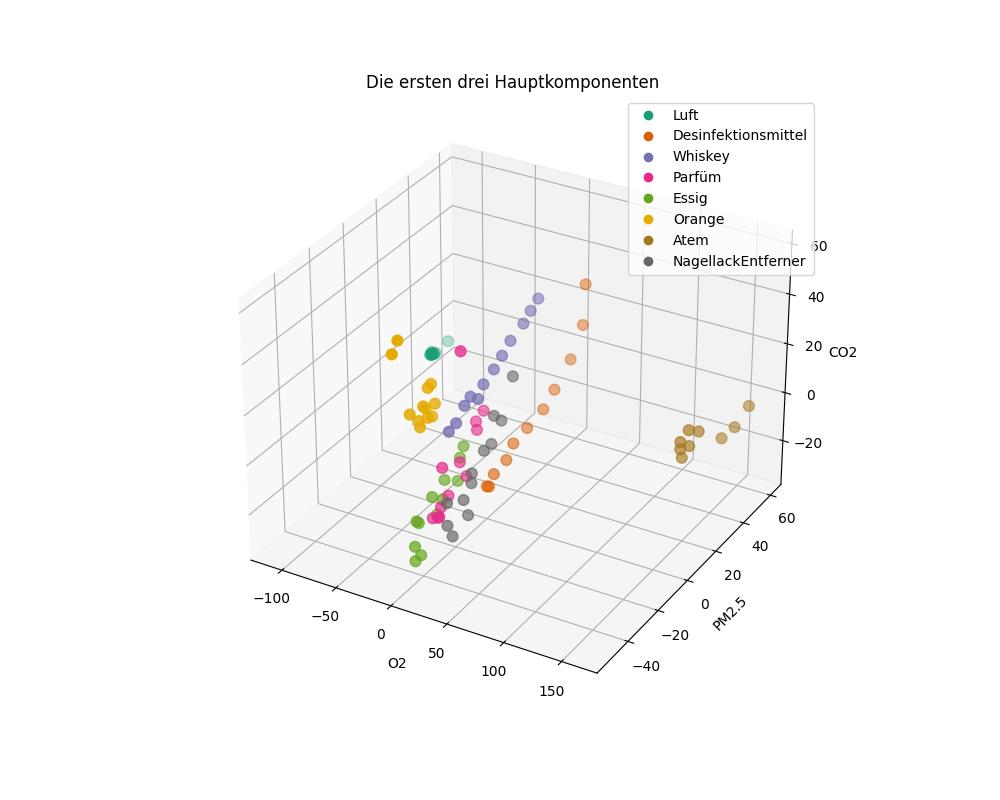
\includegraphics[scale=0.5]{Bilder/Wichtigkeit der Sensoren 3D.jpeg}
\caption{Hauptkomponentenanalyse 3D}
\end{figure} 

In dem Diagramm sind verschiedene, voneinander abgrenzbare Cluster zu erkennen. Im Zusatz \ref{Hauptkomponentenanalyse-2D} befindet sich noch eine zwei-Dimensionale
Ansicht, die vielleicht etwas übersichtlicher ist. Man kann außerdem sehen, dass manche Gerüche ziemlich schwach sind, weshalb 
sie sehr nahe an den Messungen von normaler Luft sind. Dazu zählen vor allem feste Lebensmittel wie Orangen, die einfach in ihrer Geruchsstärke vergleichsweise schwach sind.
Anscheinend haben flüssige Stoffe durch ihre Nähe zum gasförmigen Aggregatzustand in der Regel einfach eine höhere Geruchsintensität. Ich habe nämlich
zwar noch probiert andere Gerüche wie Zitrone, Muskatnuss, Tandoori, Curry und Käse zu messen, die Ausprägung von diesen Gerüchen war aber immer extrem gering.
Dadurch wurden oft Schwankungen in normaler Luft mit diesen verwechselt, weshalb ich die Gerüche nicht in die Liste der zuverlässig erkennbaren aufnehmen wollte.\\
Dem Ergebnis der Hauptkomponentenanalyse ist zudem zu entnehmen, dass man vermutlich auch eine kleinere
Version der E-Nase bauen könnte, die mit weitaus weniger Sensoren auskommt. Das würde nicht nur die Kosten senken, sondern vermutlich auch noch die Erkennung von 
viel mehr Gerüchen ermöglichen. Denn wenn ich weniger Sensoren einbauen würde, könnte ich auch einen kleineren Zylinder benutzen. In diesem wäre dann die Distanz zwischen dem zu messendem Stoff
und der Sensorik viel kleiner. Der Vorteil wäre hier, dass frische Lebensmittel normalerweise nur riechbar sind, wenn man sehr nahe an diese herangeht. Den Effekt könnte ich dann so ebenfalls
ausnutzen, wodurch die Sensoren den Geruch intensiver wahrnehmen könnten.\\
Vielleicht erinnern Sie sich ja noch an den in der Einleitung erwähnten "`smell.inspector"' ? Um die Qualitäten meiner eigenen E-Nase ungefähr abzuschätzen, habe ich diesen gekauft
um die beiden vergleichen zu können. Es stellte sich aber heraus, dass man mit dem smell.inspector lediglich Messungen machen kann, während die angepriesenen KI noch in der 
Entwicklung steht. Es ist mir mit deren Software also nicht möglich, ebenfalls Gerüche zu klassifizieren. Das Unternehmen verspricht immerhin, bald zumindest Kaffee erkennen zu können. 
Dafür braucht es wohl aber noch mehr Trainingsdaten, die anscheinend vorerst die Käufer hinschicken sollen \ref{SmartNanotubes E-Mail}. Wie lange das noch dauern wird,
ist bedauerlicherweise nicht angegeben.\\
Doch auch wenn es noch keine Erkennung von Gerüchen für den smell.inspector gibt, scheint das Gerät laut der Unternehmens-Website auch mit dem Arduino und Raspberry Pi kompatibel zu sein.
Es gibt dazu vonseiten des Herstellers aber keine weitere Dokumentation. Ich konnte immerhin zumindest mit dem von mir gekauften 
Produkt feststellen, dass der smell.inspector die Daten über eine serielle Verbindung sendet. Es wäre in der Zukunft also möglich, dass ich die Daten vielleicht selber empfange
(ohne zu wissen, wofür diese stehen) und meine eigene Künstliche Intelligenz damit trainiere.


\subsection{Erweiterung der Messtechnik}
Wie bereits beschrieben, sind die meisten Sensoren, die ich in dem Sensor-Array verbaut habe, auf das Messen von gefährlichen und meist auch für uns Menschen geruchlose Gase
spezialisiert. Es gibt momentan nur den VOC Sensor, welcher den ungefähren Anteil an organischen Substanzen in der Luft abbilden kann. Diese sind vor allem in den Gerüchen von Nahrungsmitteln 
enthalten. Ich denke daher auch über eine Verbesserung nach, welche das Erkennen von diesen erweitert. Sensoren, die wie der VOC Sensor auf organische Substanzen ausgerichtet sind,
gibt es allerdings kaum. Für solche Zwecke müsste ich deshalb die Spektroskopie heranziehen. Dabei werden von
Lasern Lichtquanten mit unterschiedlicher Wellenlänge emittiert, welche mit bestimmten Molekülen interagieren. Man kann somit, wenn das Licht reflektiert wird, messen, welche Lichtquanten
absorbiert wurden. In gewisser Weise sendet man also Licht aus und schließt dann aus den Teilen, welche nicht wiederkehren, auf die Anwesenheit von bestimmter Materie. 
Dies ist ein sehr physikalischer Prozess, auf den ich deshalb nicht weiter eingehen möchte. Wichtig ist nur, dass man damit insbesondere (organische) Kohlenstoffverbindungen messen kann.
Das Ergebnis von einer solchen Messung kann man anschließend grafisch darstellen und danach mit zahlreicher Stoffen vergleichen. Die jeweiligen Absorbtionsspektren von theoretisch messbaren
Stoffen sind online zu finden \autocite{InfrarotSpektrum} \autocite{InfrarotSpektrum2} \autocite{FTIRSpektrum}.
Mithilfe dieser Technologie könnte man Proben noch detaillierter untersuchen. Das Hinderliche ist derzeit nur, dass ich die notwendige Sensorik
nicht einfach genauso wie die anderen Sensoren in den Zylinder einbauen kann. Für eine Umsetzung wäre noch eine zweite Kammer notwendig, in die dann das Gas weitergeleitet wird.
Denn da die Spektroskopie mit Licht arbeitet, müssten die Kameras, welche zur Wiederaufnahme des Lichtes dienen, sehr gut von anderweitiger elektromagnetischer Strahlung 
abgeschirmt werden. Etwas simpler gesagt: Es muss dunkel sein. Ideal wäre dabei ein schwarzes Gehäuse, zum Beispiel per 3D-Druch angefertigt, in dem dann das Spektroskop platziert wird. 
Wenn der VOC Sensor dann eine hohe Konzentration von organischen Substanzen erkennt, könnte der Inhalt des durchsichtigen Zylinders über einem Schlauch in das Spektroskopie-Gehäuse gesogen werden,
wo es dann noch einmal untersucht wird.\\
Die Umsetzung eines Spektroskops kann man auf verschiedene Arten und Weisen ermöglichen. Diese unterscheiden sich hauptsächlich darin, wie präzise und dementsprechend teuer sie sind. 
Die RAMAN-Spektroskopie beispielsweise würde vermutlich die meisten Informationen bereitstellen können. Eine solche Anwendung würde aber, wenn überhaupt, in ferner Zukunft liegen. 
Die Gerätschaften sind hier äußerst kostspielig, meist im vierstelligen Bereich, man müsste sich also eine eigene, kostengünstigere
Variante bauen. Es gibt dazu auch Anleitungen \autocite{RamanBauTheorie} \autocite{RamanPi}, ein Bau würde aber vermutlich sehr aufwendig und langwierig sein. Um einiges vielversprechender 
ist die Verwendung von Infrarot (IR) und Ultraviolett (UV) emittierende Spektroskopen. Dies sind zwar ebenfalls nicht billig, aber um einiges preiswerter \autocite{UV_IR_Sensor}, sie sind
noch im zweistelligen Bereich. Da ich für die Erkennung von Gerüchen keine akribisch genauen Messwerte brauche, würden diese auch vollkommen ausreichen. Die Messergebnisse der Sensoren
könnte ich anschließend innerhalb der Software als diskrete Serie von Messwerten, also einem Linien-Diagramm ähnlich, darstellen. Danach könnte ein Algorithmus das erhaltende Spektrum
mit denen von verschiedenen Stoffen vergleichen und somit auf den Inhalt des schwarzen Gehäuses schließen. Eine weitere Möglichkeit besteht darin, dass ich das Spektrum ohne weitere Verarbeitung 
direkt in die künstliche Intelligenz speise. Die Herausforderung bei dieser Messmethode wäre wahrscheinlich wieder einmal die Beseitigung von Störungen, wobei die erstgenannte
Verarbeitungsmethode vielversprechender wäre.\\
Um eine höhere Auflösung zu erreichen, wäre zudem eine Erweiterung der Infrarot Spektroskopie mittels der Fourier-Transform-Infrarot (FT-IR)-Spektroskopie \autocite{FTIR} denkbar. 


\subsection{Erweiterung für industrielle Zwecke}
Ein weiteres großes Potenzial des Sensor-Arrays sehe ich in dem IoT Bereich.
Beispielsweise ist die Stadtverwaltung von Brandenburg an der Havel schon auf mich zugekommen, welche an einem Sensor-Array als Embedded Device interessiert wäre.
Insbesondere das LoRaWAN \autocite{LoRaWAN} Protokoll würde dort eine große Rolle spielen. Mit diesem kann man großflächig eingebetteten Systeme mit einem Gateway verbinden, 
die Kommunikation funktioniert hierbei über Funk. Die in der Einleitung erwähnte Anwendung zur Kontrolle und Steuerung von Belüftungssystemen würde davon im besonderen Maße profitieren. 
Man könnte eine kleine Version der E-Nase in vielen Gebäuden installieren, welche dann das Ergebnis der Erkennungssoftware weiterleiten würden. Ich hätte zudem die Chance, meine E-Nase
in dem bereits bestehenden Netz der Stadtverwaltung zu testen.\\
Um bei dem möglichen Bau von weiteren E-Nasen möglichst viele Hardware-Kosten zu sparen, würde ich für die Ausführung der Messungs-Software einen sehr schwachen Computer 
wie den Raspberry Pi Zero nehmen (oder Alternativen, falls dieser zu dem Zeitpunkt wieder/noch ausverkauft ist). Es wäre sogar möglich, 
die Festplatte, in diesem Fall die SD-Karte einzusparen, indem man das gesamte Betriebssystem als auch die Software
in den RAM lädt. Der Computer wäre dann zeitlich außerdem nicht mehr von dem TBW (Total Bytes Written) Limit der Festplatte abhängig. Nebenbei würden auch Stromkosten von dem
fehlenden Hardware-Teil gespart werden, auch wenn beide Effekte zugegebener Maßen eher gering ausfallen würden. Dennoch wäre eine RAM-Disk sehr praktisch.
Zum Beispiel verbraucht Tiny-Core Linux \autocite{piCore} nur wenige Megabytes, man könnte aber natürlich auch zu 
Real Time Operating Systems (RTOS) greifen, wenn ein bestimmter Anwendungsfall dies benötigt. Sollte der Computer in bestimmten Anwendungsfällen als Server fungieren oder anderweitig mit dem
Internet verbunden sein, wäre allerdings ein weitaus höherer Sicherheitsstandard erforderlich. Eine Übernahme durch Malware wie "`Mirai"' \autocite{Mirai} wäre nämlich ziemlich kritisch, insbesondere
wenn die Geruchserkennung zur Überwachung von gefährlichen Gasen dienen soll. In diesem Fall wäre womöglich das Nutzen von Arch Linux von Vorteil, da dieses ebenfalls von Hause aus einen
geringen RAM-Verbrauch hat. Auch hier gäbe es optional ein Realtime kernel patchset. Das Hardening, also das Verbessern der Sicherheit, 
wäre zudem durch das Vorhandensein von systemd oder des hardened-kernel Packages weitaus einfacher. Dazu kommt noch die Möglichkeit von Mandatory Access Control (MAC) \autocite{MAC},
wodurch SElinux oder im Falle von Arch Linux AppArmor \autocite{SElinuxAndAppArmor} zusätzliche, die meisten Standards übertreffende Sicherheit gewährleisten könnte.\\
Das Laden von allen Ressourcen in den RAM wäre außerdem nicht nur kostengünstiger, sondern würde auch die I/O Leistung erhöhen.\\
Natürlich ist die einzige Krux, dass ein günstiger Computer wenig RAM hat, 
im Falle eines Raspberry Pi Zeros wären es 512 MB \autocite{PI0Specs}. Zwar würde Arch oder sogar Tiny Core Linux nur einen Bruchteil davon beanspruchen, die limitierenden Faktoren
währen aber vermutlich die darauf laufenden Programme. Die Messungs-Software benötigt eine JVM. Die Teile des Codes, welche für die GUI verantwortlich sind, könnte ich allerdings vorher 
entfernen. Nur mit dem zusätzlichen Python-Interpreter und den TensorFlow Bibliotheken könnte es sehr eng werden – diese verbrauchen zusammen mehrere Gigabytes.
Hier kommt mir ein Projekt zugute, welches ich letztes Jahr umgesetzt habe. Ich habe dort ein Neuronales Netz von Grund auf selbst programmiert, geschrieben in Java und ohne 
ergänzende Bibliotheken. Den Code von diesem Programm habe ich mittlerweile einem starken Refactoring unterzogen. 
Das zu einem Punkt, an dem ich behaupten würde, dass der Quelltext nur noch wenig mit der alten Version gemeinsam hat. Jedenfalls habe ich schon zu Testzwecken den Teil dieses 
Projektes extrahiert, welcher für das Laden des gespeicherten Models und dessen Gewichten zuständig ist, sowie für das anschließende Ausführen des Neuronalen Netzes.
Der Code ist dadurch extrem kompakt, schließlich beinhaltet er nur das absolut Nötigste. Diese Methoden habe ich in die Messungs-Software integriert. Ich kann nun also
die KI extern trainieren und anschließend die gelernten Gewichte in dem Daten-Ordner der Messungs-Software speichern. Diese ist damit komplett unabhängig von Python. 
Um trotzdem von der immensen Leistung TensorFlow's zu profitieren, habe ich mir die Wahl der Hyperparameter von Keras-Tuner abnehmen lassen. Das ist ein normales Package, welches man
mittels pip installieren kann. Dadurch, dass Keras in TensorFlow integriert ist, kann man diese Bibliothek nutzen, um ein sogenanntes "`HyperModel"' zu erstellen. Bei diesem kann ich angeben, 
welche Hyperparameter von Keras ausprobiert werden sollen. Das reicht von relativ simplen Dingen wie der Batch-Size bis hin zu der Anzahl von Hidden Layern, deren Neuronen-Anzahl
und Aktivierungsfunktion. Man hat dort die Wahl zwischen verschiedenen Algorithmen. Ich habe mich für den "`Hyperband"' \autocite{Hyperband} Algorithmus entschieden, welcher gegenüber
einer jedes Mal zufälligen Wahl an Hyperparametern versucht, den Prozess deutlich zu verkürzen (ohne hier mehr in das Detail zu gehen). Ich bekomme somit nach einigen Durchläufen die optimale
Kombination aus Hyperparametern, um ein zuvor definiertes Lernziel so gut wie möglich zu erreichen. In meinem Fall ist das die Genauigkeit auf den Trainingsdaten.\\
Durch diese Konfigurationsschritte wäre es also möglich, die E-Nase auch in größeren Maßstäben zu verwenden. Ich habe essenzielle Teile, wie das Laden in den RAM
und weiteres, bereits erfolgreich ausprobiert. Auch den Teil mit der Künstlichen Intelligenz konnte ich schon in die Messungs-Software integrieren. Ob es zu diesem Anwendungsfall kommt,
wird sich im weiteren Austausch sehen lassen.

\section{Fazit}
Das automatische Erkennen von Gerüchen funktioniert mit meiner E-Nase also für viele Stoffe. Mithilfe des von mir gebauten Sensor-Arrays
kann man Messungen von Gerüchen nehmen, welche meine Software anschließend mit hoher Genauigkeit zuordnen kann. Auch wenn dies nicht mit allen Gerüchen möglich ist, 
liegt das eher an der dazu noch fehlenden Messtechnik. Eine Verbesserung würde eine zweite Version meiner E-Nase darstellen. Insbesondere Sensoren, die sich mithilfe 
der Hauptkomponentenanalyse als größtenteils redundant herausgestellt haben, könnten dabei entfernt oder ersetzt werden. 
Dennoch ist die E-Nase vor allem im Vergleich mit den derzeitigen industriellen Produkten sehr attraktiv:
Es sind weitaus mehr Gerüche erkennbar, als es der smell.inspector kann. Vor allem der Preis spricht, trotz der vielen Sensoren, für sich. Während der 
smell.inspector knapp 500 Euro kostet, komme ich bei dem Bau auf Kosten von ungefähr 200 Euro, wenn man den Mini-Computer nicht mitrechnet.\\
Zusammenfassend ist das Projekt aus meiner eigenen Sicht definitiv gelungen. Als erster Prototyp konnte 
ich Schwachstellen finden, die ich in der Zukunft verbessern kann. Für den Einsatz in der Praxis überzeugt meiner Meinung allerdings jetzt schon der Preis, das einfache 
selbstständigen Hinzufügen von Gerüchen mittels der Grafikoberfläche und die äußerst vielfältigen Anwendungsmöglichkeiten.

\newpage

\printbibliography[heading=bibintoc, title={Quellen- und Literaturverzeichnis}]

\appendix
%\newpage

\section{Ergänzungen}
\subsection{MQ-Sensoren}

\begin{table}[H]
\centering
\rowcolors{2}{gray!10}{gray!40}
\begin{tabular}{cc}
Name & Gas \\
\hline
MQ-2 & Methan, Butan, LPG, Rauch \\
MQ-3 & Alkohol, Ethanol, Rauch \\
MQ-4 & Methan, CNG Gas (komprimiertes Erdgas) \\
MQ-5 & Erdgas, LPG (Autogas) \\
MQ-6 & LPG (Autogas), Butan \\
MQ-7 & Kohlenmonoxid \\
MQ-8 & Wasserstoffgas \\
MQ-9 & Kohlenmonoxid, entflammbare Gase \\
MQ-131 & Ozon Gas \\
MQ-135 & Benzol, Alkohol, Rauch\\
MQ-136 & Schwefelwasserstoffgas\\
MQ-137 &  Ammoniak\\
MQ-138 &  Benzol, Steinkohlenteeröl (Toluol), Aceton, Propan, Formaldehyd, Wasserstoffgas\\
MQ-214 &  Methan, Erdgas\\
MQ-216 & Erdgas, Kohlegas\\
MQ-303A &  Alkohol, Ethanol, Rauch\\
MQ-306A &  LPG (Autogas), Butan\\
MQ-307A &  Kohlenmonoxid\\
MQ-309A &  Kohlenmonoxid, entflammbare Gase\\
MG811 & Kohlenstoffdioxid\\
AQ-104 & Luftqualität\\
AQ-2 & entflammbare Gase, Rauch\\
AQ-3 & Alkohol, Benzin\\
AQ-7 & Kohlenmonoxid\\
\end{tabular}
\caption{Alle MQ-Sensoren}
\label{MQ-Tabelle}
\end{table}

\bigskip
Alle Sensoren stammen von \autocite{MQSensoren}.


\label{PCA}
\subsection{Die wichtigsten Hauptkomponenten}

\begin{table}[H]
\centering
\rowcolors{2}{gray!10}{gray!40}
\begin{tabular}{cc}
Sensor & Hauptkomponent \\
\hline
CO2 & 0,635 \\
PM2.5 & 0,220 \\
MQ-8 & 0,002 \\
MQ-5 & 0,001 \\

\end{tabular}
\caption{Die wichtigsten Hauptkomponenten}
\label{PCA-Tabelle}
\end{table}


\label{Hauptkomponentenanalyse-2D}
\subsection{Hauptkomponentenanalyse 2D}

\begin{figure}[H]
\centering
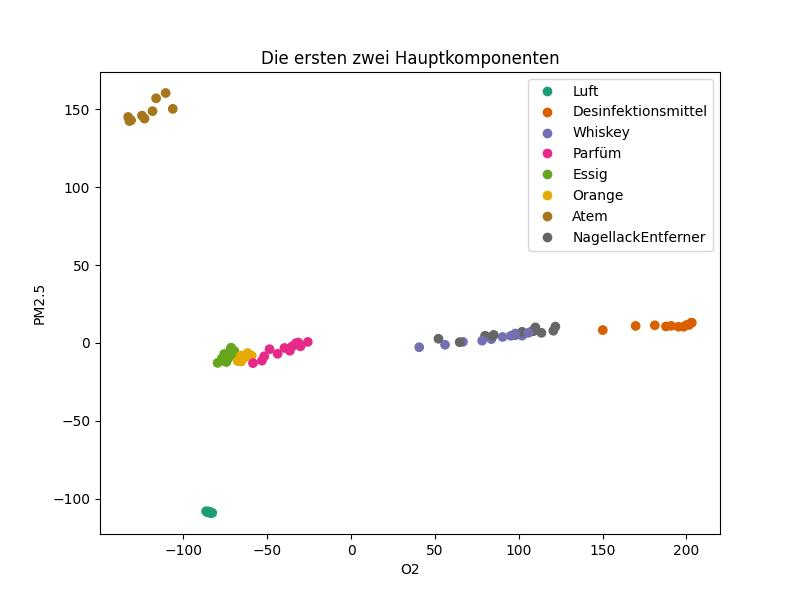
\includegraphics[scale=0.9]{Bilder/Wichtigkeit der Sensoren 2D.jpeg}
\caption{Hauptkomponentenanalyse 2D}
\end{figure}


\label{SmartNanotubes E-Mail}
\subsection{SmartNanotubes E-Mail}

\begin{figure}[H]
\centering
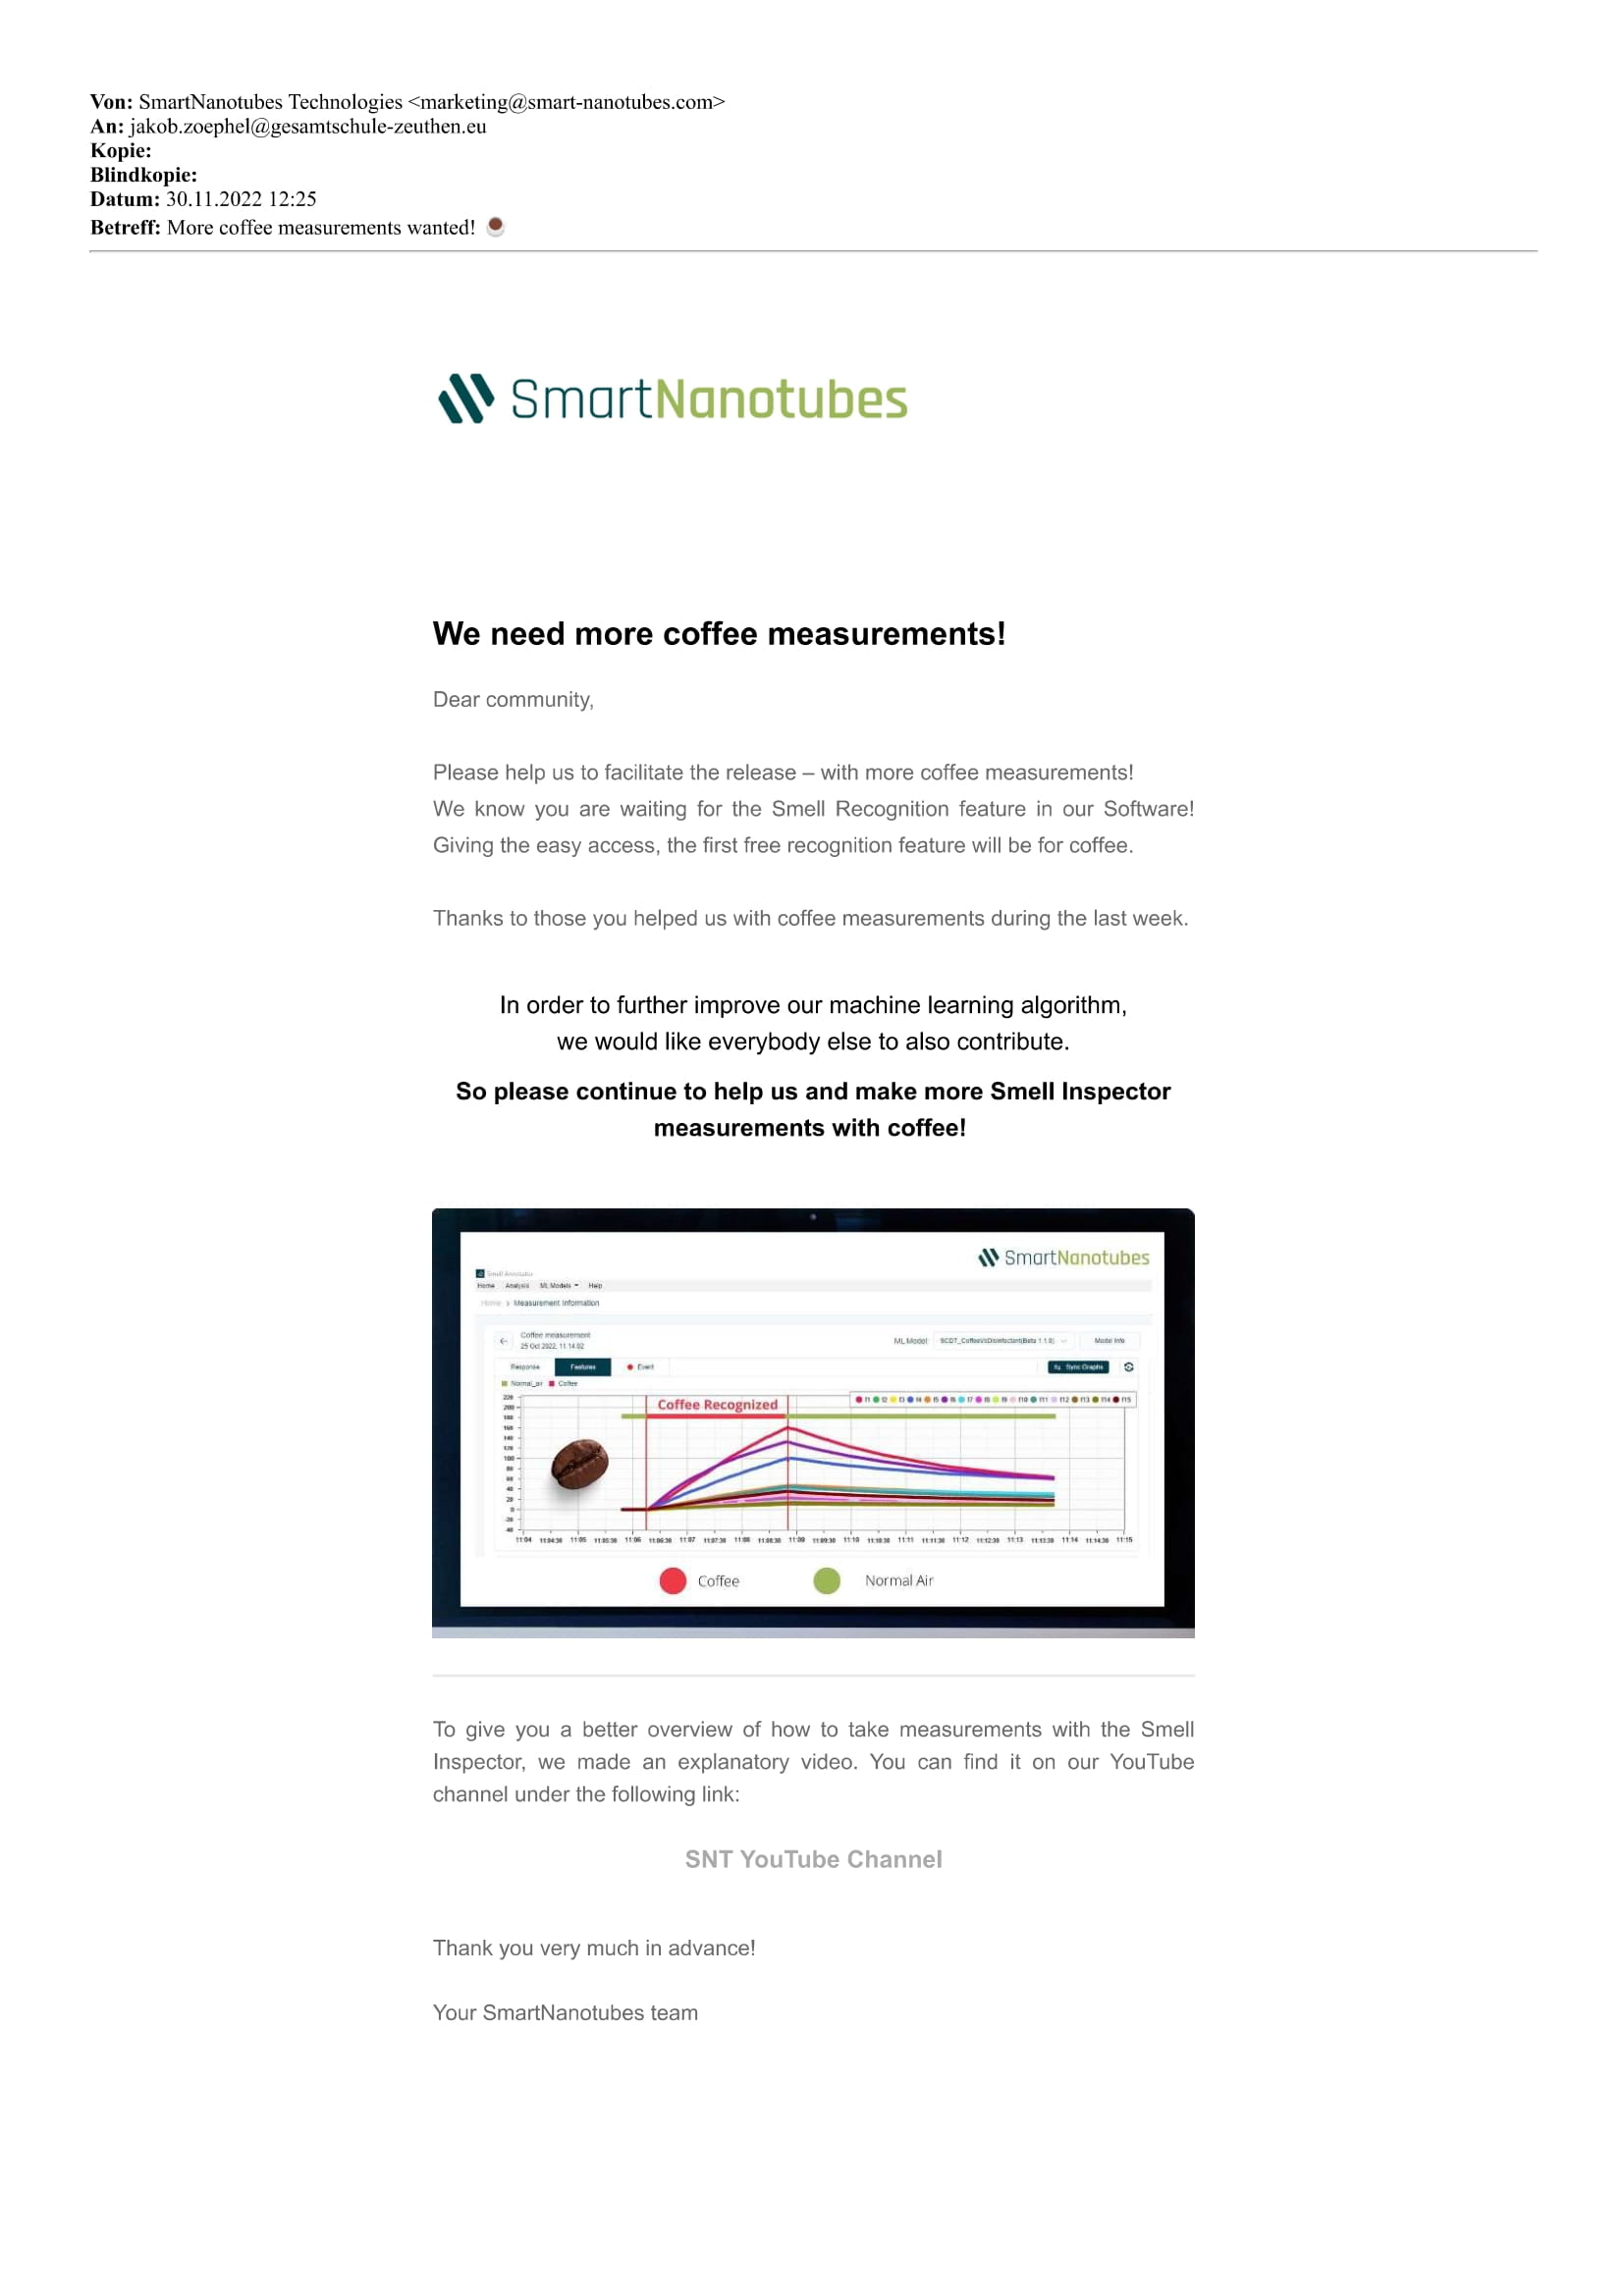
\includegraphics[scale=0.26]{Bilder/E-Mail-NanoTubes.jpg}
\caption{SmartNanotubes E-Mail}
\end{figure}

\end{document}